\documentclass[conference]{IEEEtran}
\IEEEoverridecommandlockouts
\usepackage{cite}
\usepackage{subfigure}
\usepackage{hyperref}
\usepackage{amsmath,amssymb,amsfonts}
\usepackage{algorithmic}
\usepackage{graphicx}
\usepackage{textcomp}
\usepackage{xcolor}
\usepackage{float}
\pagenumbering{arabic}
\pagestyle{plain}
\def\BibTeX{{\rm B\kern-.05em{\sc i\kern-.025em b}\kern-.08em
    T\kern-.1667em\lower.7ex\hbox{E}\kern-.125emX}}
    
\begin{document}

\title{Lab Report: TiO$_2$ dye sensitized solar cells}

\author{\IEEEauthorblockN{1\textsuperscript{st} Sebastiaan Vanspauwen}
\IEEEauthorblockA{\textit{Faculty of Industrial Engineering} \\
\textit{Student number: 1540883}\\
Diepenbeek, Belgium \\
sebastiaan.vanspauwen@student.uhasselt.be}
\and
\IEEEauthorblockN{2\textsuperscript{nd} Jeffrey Gorissen}
\IEEEauthorblockA{\textit{Faculty of Industrial Engineering} \\
\textit{Student number: 1436845}\\
Maaseik, Belgium \\
jeffrey.gorissen@student.uhasselt.be}
\and
\IEEEauthorblockN{3\textsuperscript{rd} Turpal Dadaev}
\IEEEauthorblockA{\textit{Faculty of Industrial Engineering} \\
\textit{Student number: 1952978}\\
Dilsen Stokkem, Belgium \\
turpal.dadaev@student.uhasselt.be}
}

\maketitle
\thispagestyle{plain}

\begin{abstract}
The goal of this lab is to understand how to create TiO$_2$ dye-sensitized solar cells and to test their efficiency. This includes choosing a type of natural dye, backed by research, that would yield the best results. After choosing the dye, the solar cells are built and tested. The testing is performed on a switchboard and data processing software (LabView). 
\\
\end{abstract}

\begin{IEEEkeywords}
TiO$_2$, dye, sensitized, solar, cell
\end{IEEEkeywords}

\section{Introduction}\label{intro}
The sun is the main source of energy for planet earth. The sun provides light and warmth for all living organisms. Humans take this a step further and use the energy of the sun to make solar energy. Solar energy is a clean and renewable energy source.

\subsection{Solar cell}
To capture the energy of the sun, solar cells have been invented. Solar cells convert the energy from the photons of the sun into electrical energy. This can be used to power all kinds of electronic devices. Not all of the energy that reaches a solar cell gets converted into electrical energy. Therefore, a lot of research is being done to improve the efficiency of existing solar cells.\\

\subsubsection{Silicon solar cells}
Silicon solar cells are either multi-crystalline silicon (multi-Si) consisting of small crystals, or mono-crystalline silicon (mono-Si), a continuous crystal. These cells are assembled into solar panels, as seen in Figure \ref{fig:monomulti}, as part of a photo-voltaic system to generate solar power from sunlight.\\

\begin{figure}[h]
\centering
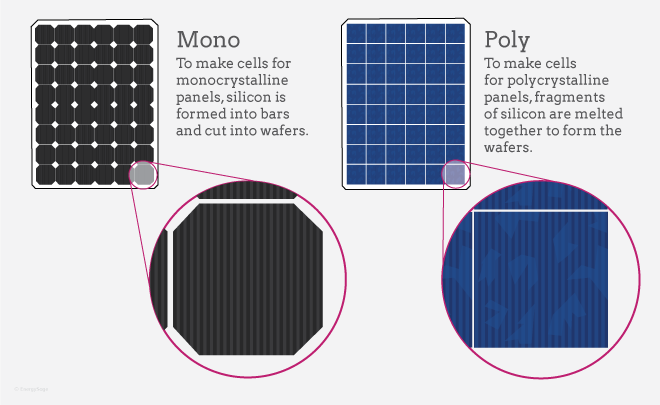
\includegraphics[width=80mm]{monomulti.png}
\caption{The visual difference between mono- and multi-Si panels. \cite{monomulti}}
\label{fig:monomulti} %use label to refer to it in later text
\end{figure}

Solar cells made of crystalline silicon are the most common type up to the present time. They are often called conventional, traditional, or first-generation solar cells, as they were developed in the 1950s.\\

\subsubsection{TiO$_2$ dye-sensitized solar cells}
A dye-sensitized solar cell (DSSC) is a budget solar cell that is part of the thin-film solar cells. It is a semiconductor formed between two glass plates with a conductive coating applied to them. A layer of graphite is applied to the conductive side of one glass plate: this glass plate will form the anode or positive electrode of the solar cell; on the other glass plate a layer of TiO$_2$ is applied: this glass plate will be the cathode or negative electrode of the solar cell. Between both glass plates, an electrolyte solution is added.\\

The DSSC has some improvements over the traditional silicon cells; it is simple to manufacture with conventional roll-printing techniques, is semi-flexible and semi-transparent which increases the use-cases for this type of solar cells, and most of the used materials are budget-friendly.\\

The objective of this lab is to fabricate a DSSC using a natural dye. In this case, beetroot and black tea were selected. The selection of beetroot and black tea is based on a short literature study.  For more information please refer to section \ref{ResearchDyes} Research of the dyes.\\

\section{Methods and Materials}

\subsection{Methods}
This section shows the consecutive steps that are needed to construct and evaluate a dye sensitised solar cell while following the given lab instructions. The first paragraph discusses how the solar cell is constructed. The second paragraph gives insight how to measure the I-V curve of a solar cell.\\

\paragraph{Preparation of a single solar cell}
The first step is to take two glass plates out of a box, this while wearing nitrile gloves to not leave any grease on the plates. Measure the glass plates with a multimeter so the conductive side is known. To improve the conductivity of the glass plates, it is recommended to clean the conductive side with a degreaser. After this step, it is \emph{very} import to not touch the conductive side. \\

Place both glass plates on a piece of paper with the conductive side facing upwards. To make the anode, \textit{"colour"} one of the glass plates' conductive side with a graphite pencil. This creates the positive side of the solar cell. The cathode, or negative side, takes a few more steps to make.\\ 

First, the conductive side should be taped in a way that only a few millimetres on each side are taped. When the glass plate is firmly taped to the paper, suck up a small amount of TiO$_2$ paste with a pipette. Gently drop this small amount of paste on the conductive side of the cathode (a single drop should suffice). When the paste is applied, the next step is to thin the layer by using a microscopic glass. When the layer is fully dried, carefully remove the scotch tape from the cathode. Next step is to take a piece of aluminium foil and place the cathode facing upwards on the foil. Ignite the Bunsen burner and place the aluminium foil so it heats the glass plate. Wait until the colours shifts from white to brown and back to white. When the colour shifting is done, it is important to let the glass cool down.\\

When the glass is at room temperature, submerge the cathode with TiO$_2$ paste fully into the petri dish with dye as seen in figure \ref{fig:submergingTiOHib}. After ten minutes the TiO$_2$ paste should have soaked up the dye. Wait until the solution is dry and carefully rinse, as to not wash away the sensitized TiO$_2$, with distilled water.\\


\begin{figure}[H]
\centering
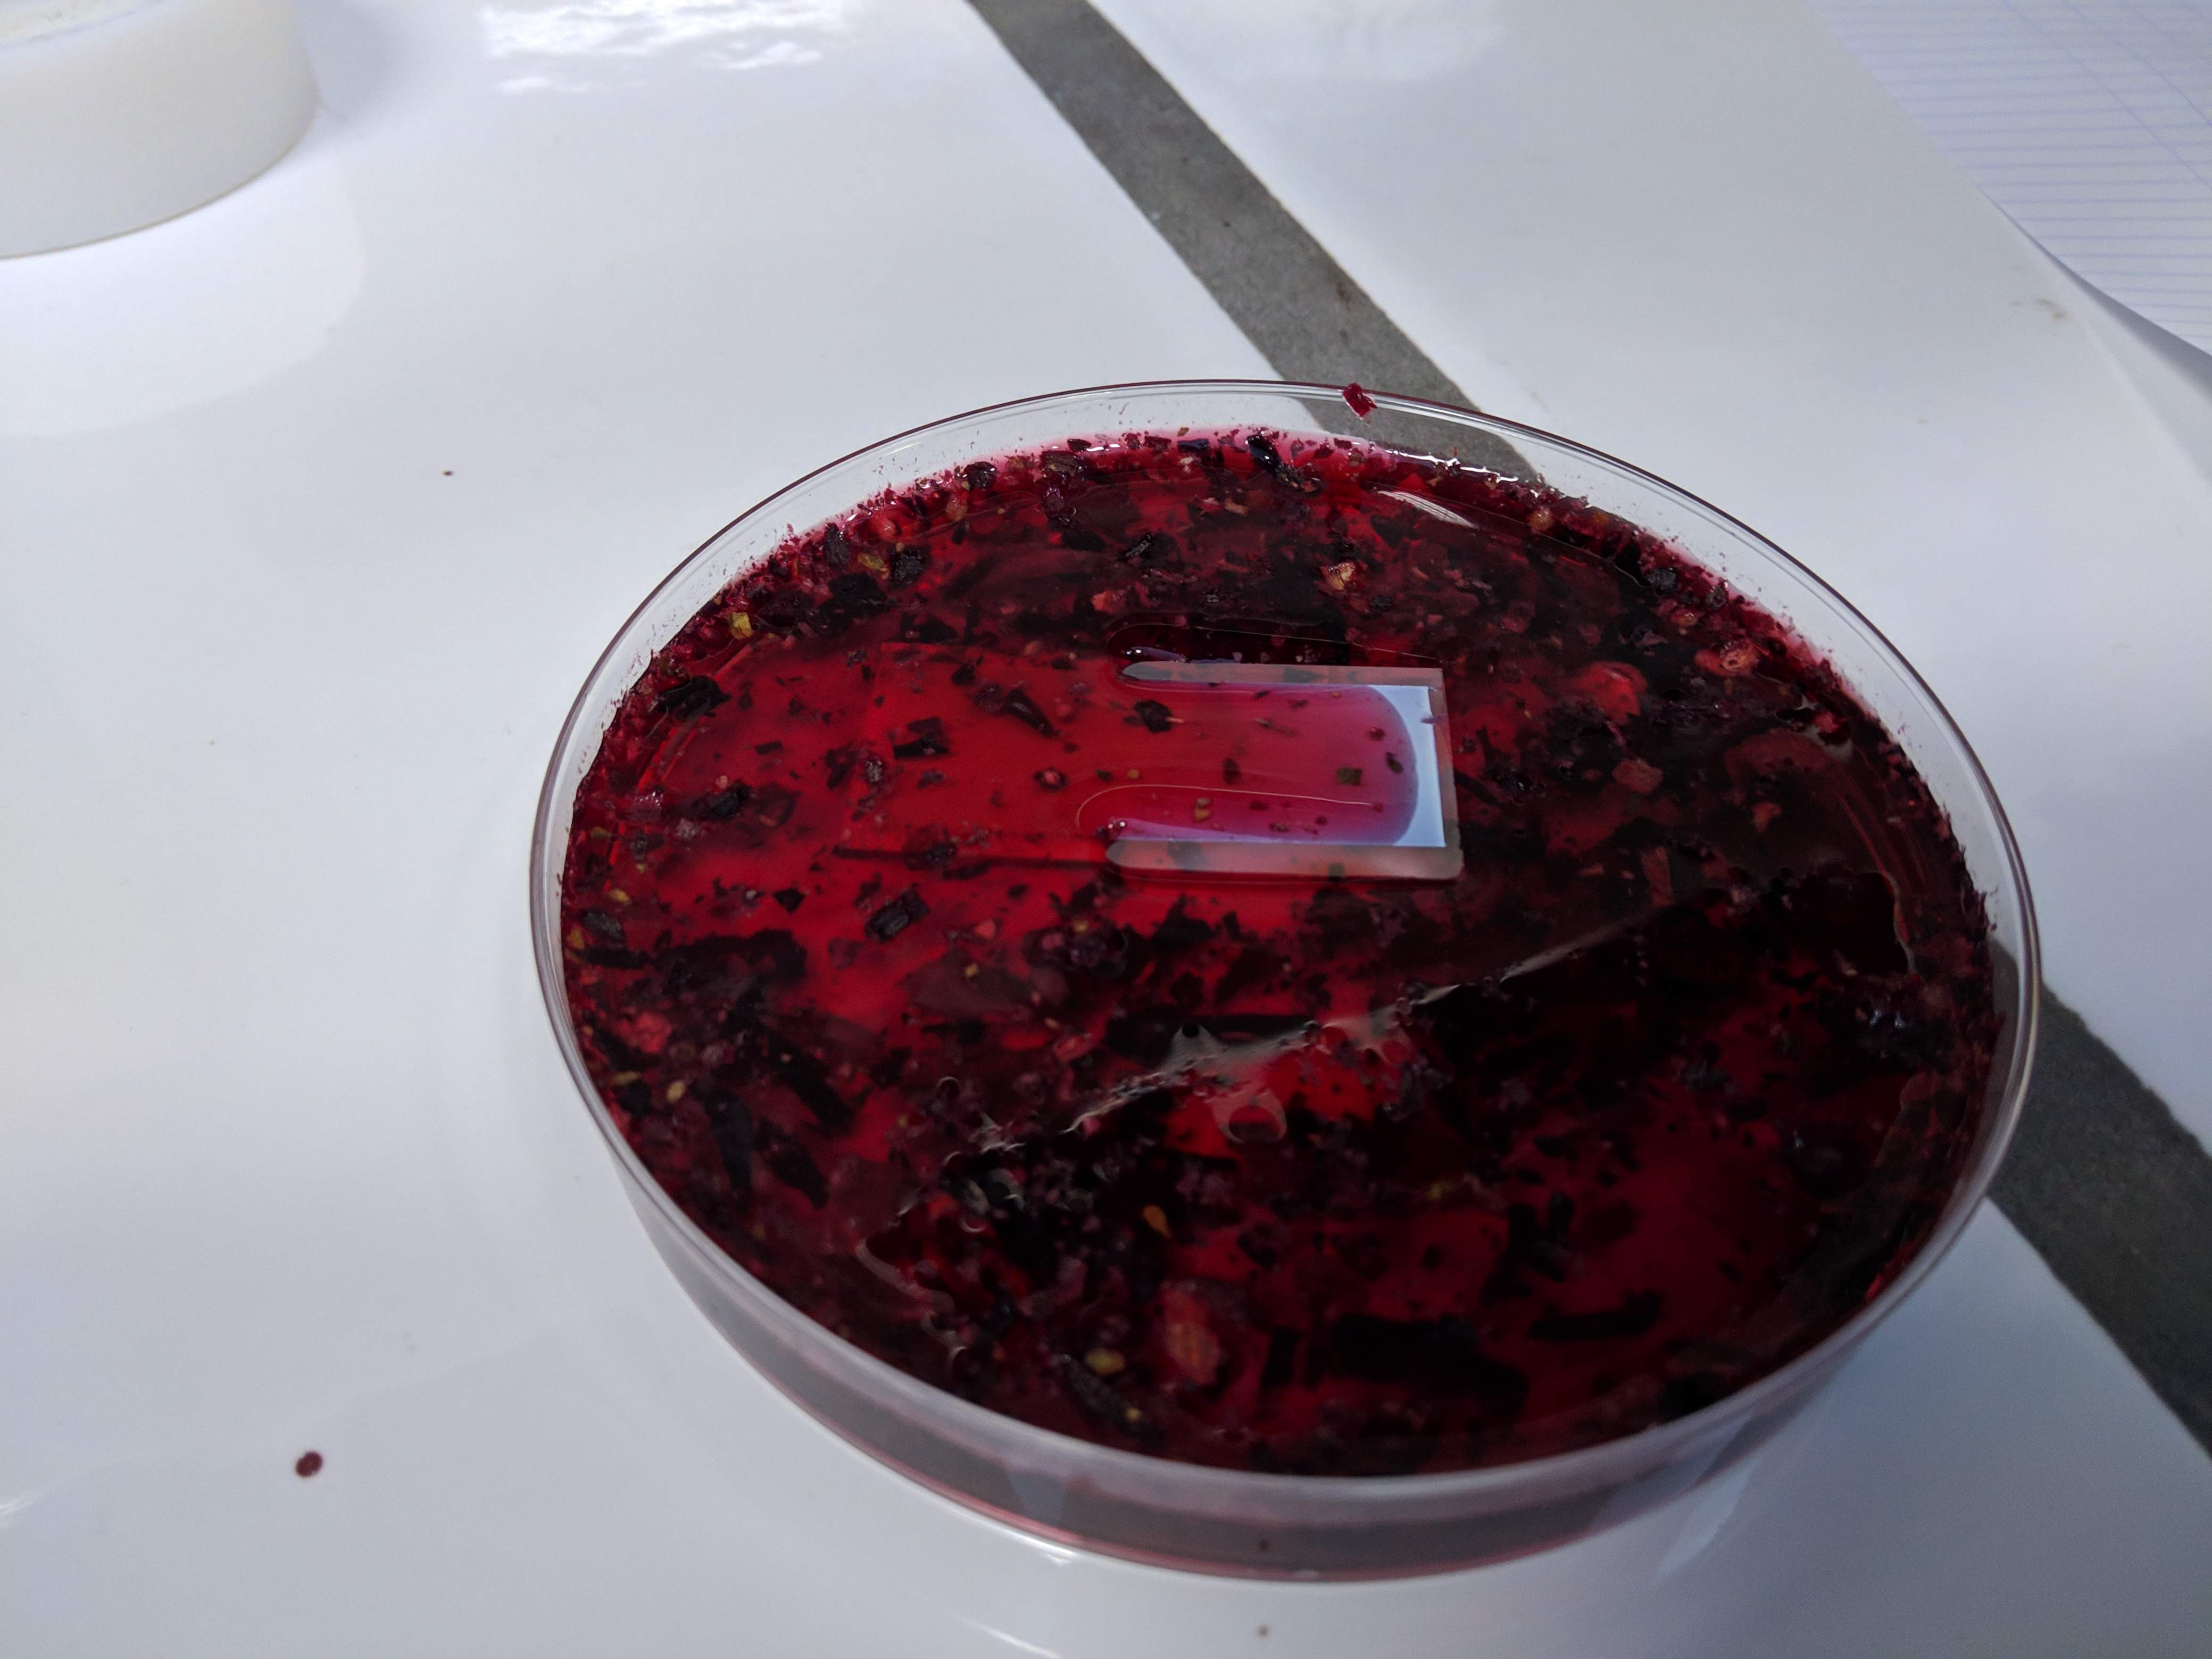
\includegraphics[width=8.0cm]{5SubmergingTiOHib.jpg}
\caption{Submerging the TiO$_2$ paste into Hibiscus dye.}
\label{fig:submergingTiOHib} %use label to refer to it in later text
\end{figure}

Both the anode and cathode are ready to create a dye sensitised solar cell. All that is left is to apply a few droplets of electrolyte solution between the two conductive sides. Bend a paperclip in a way that it will keep both glass plates together. Gently place both conductive sides so that they touch and apply the paperclip. Make sure there is some space on both sides to connect measurement clips.\\

\paragraph{Measurement of a single solar cell}
The test setup can be seen in fig. \ref{fig:cellmeasurement}.

\begin{figure}[H]
\centering
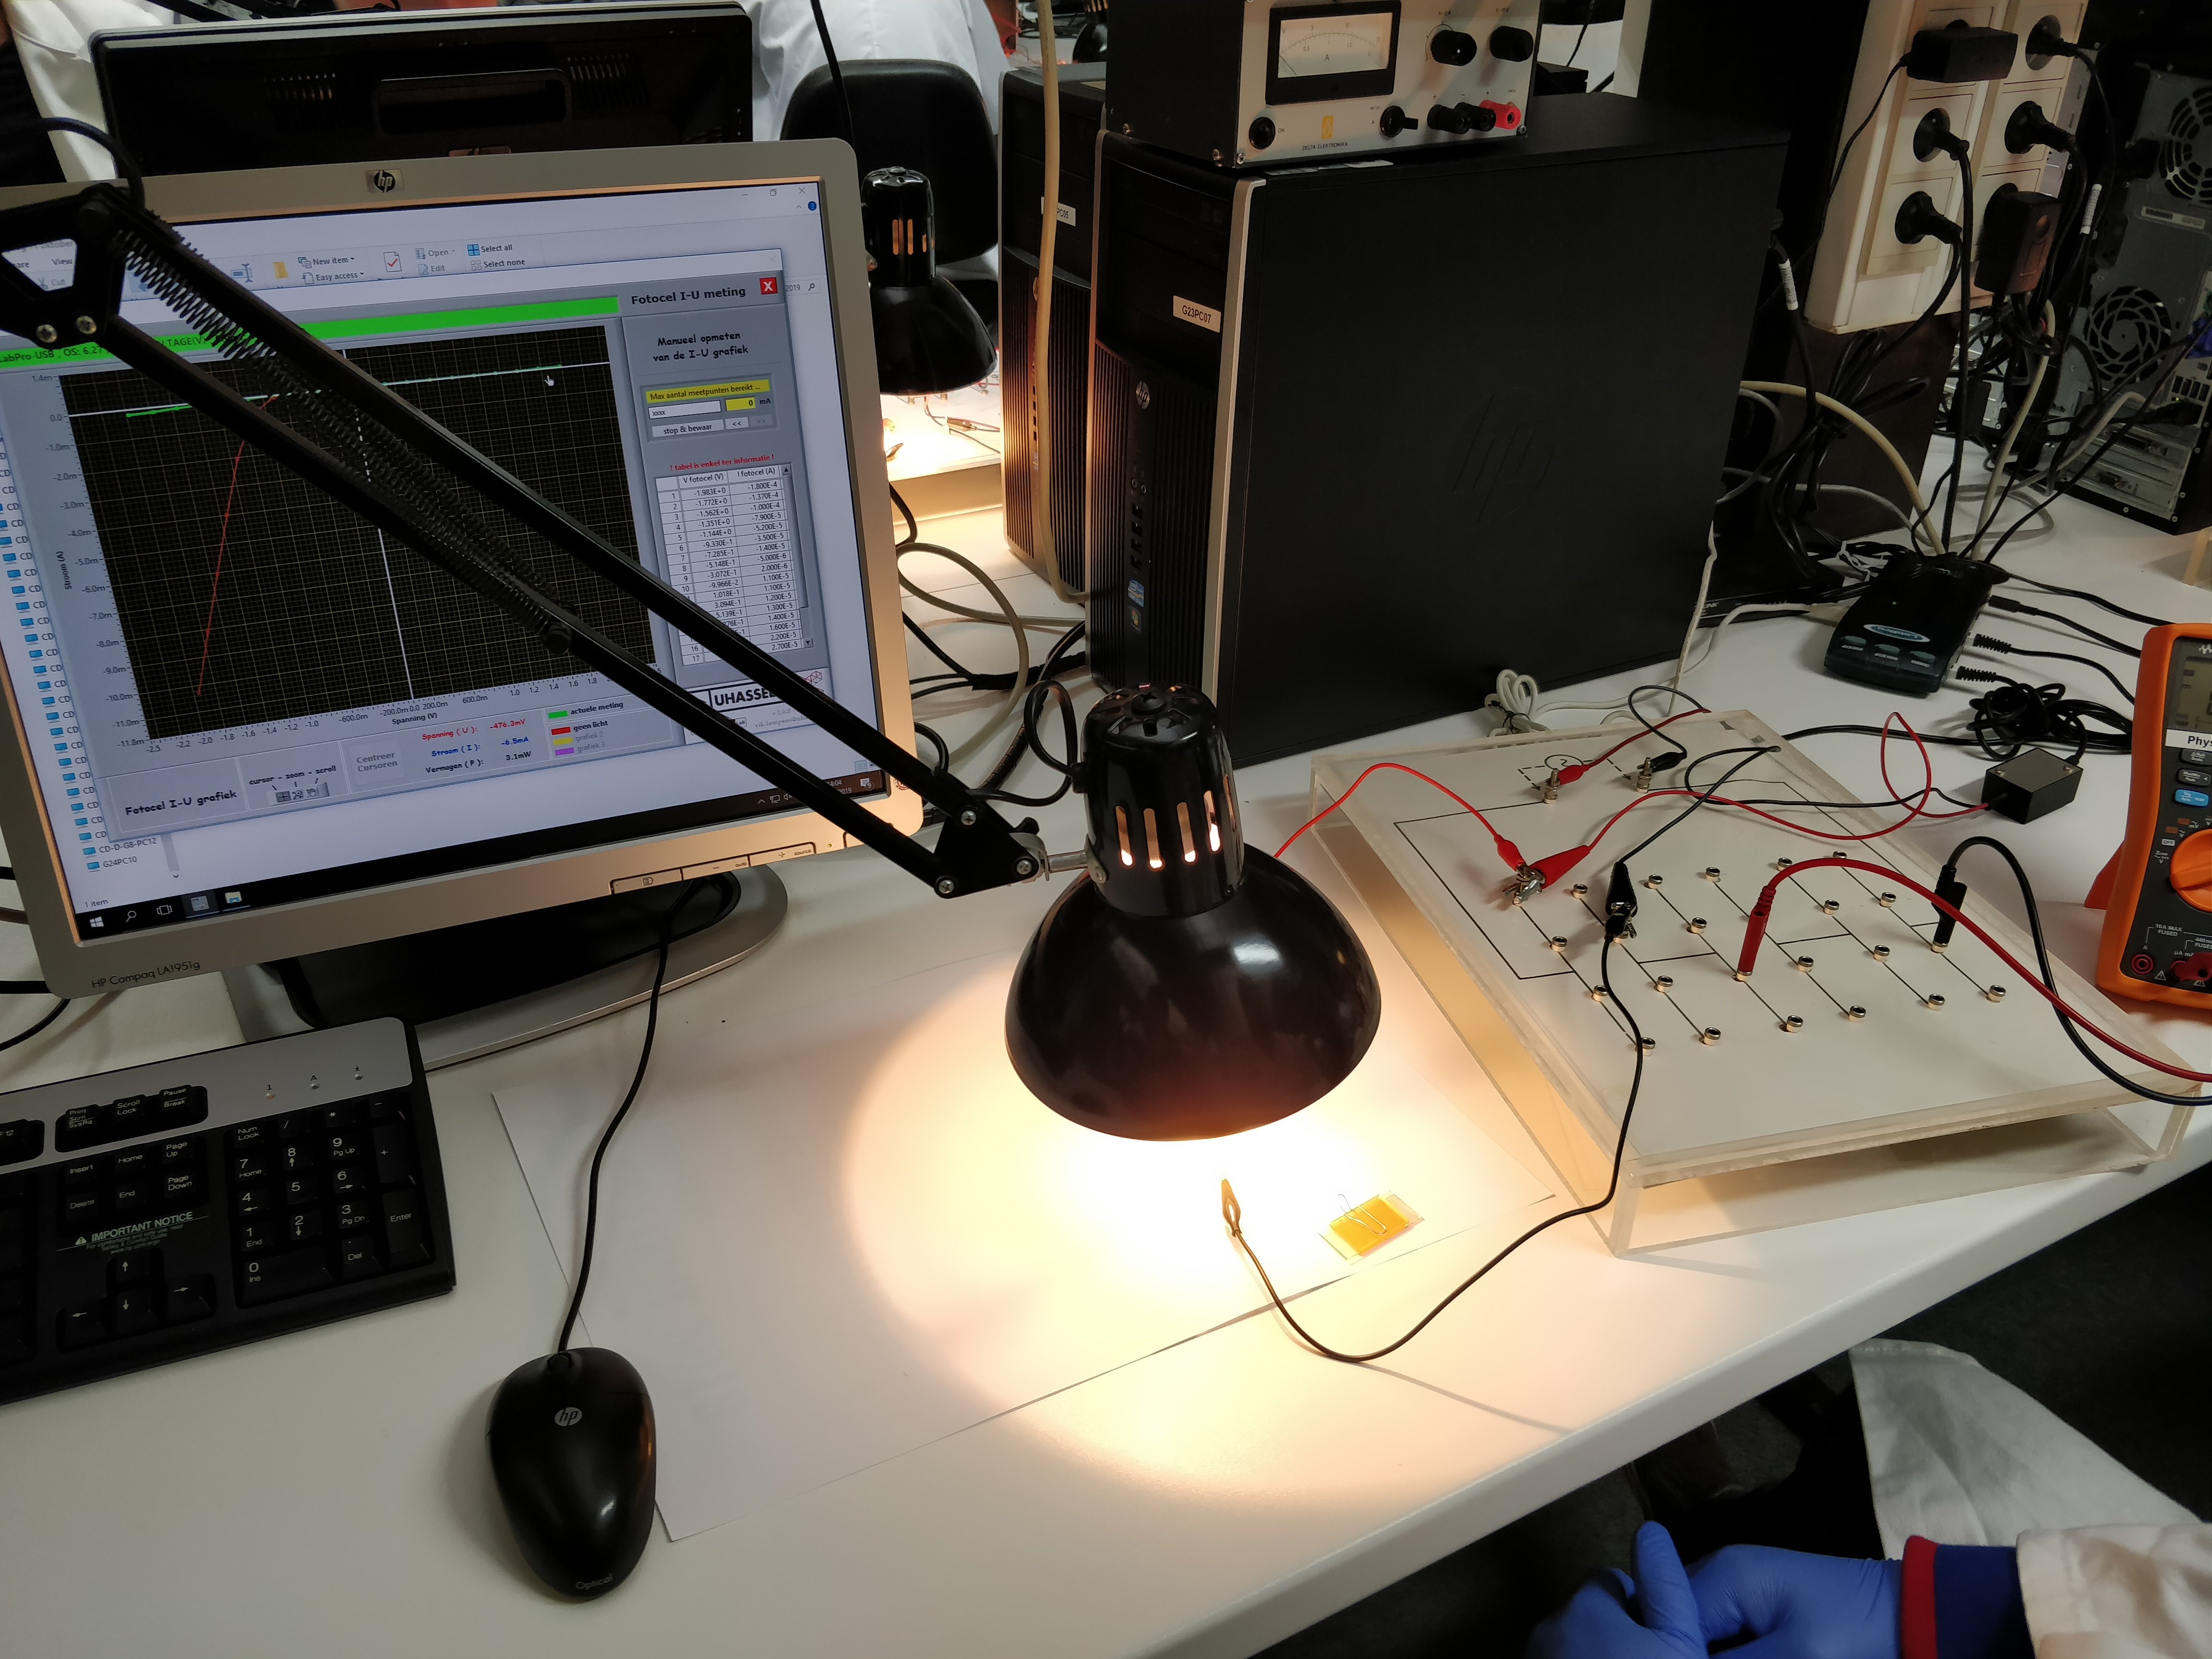
\includegraphics[width=8.0cm]{CellMeasurement.jpg}
\caption{Measurement setup.}
\label{fig:cellmeasurement} %use label to refer to it in later text
\end{figure}

\subsection{Materials}
This section contains all of the needed equipment that was needed to perform this experiment.\\
\begin{itemize}
  \item multimeter
  \item two glass plates
  \item degreaser
  \item soft cloth
  \item pencil
  \item paper
  \item adhesive tape
  \item TiO$_2$ paste
  \item pipette
  \item microscope slide
  \item Aluminium foil
  \item bunsen burner
  \item tripod
  \item wire net
  \item dye
  \item petri dish
  \item paper clip
  \item electrolyte solution
  \item (extra) water boiler
  
\end{itemize}


\section{Experimental Procedure}

\subsection{Research of the dyes} \label{ResearchDyes}
In this experiment, two different dyes were selected for testing. During the research process red turnip \textit{(Brassica rapa var. rapa)} was selected as a first dye candidate with for its (relative) high efficiency (1,70\%) \cite{redturnipeff}, low cost and high availability in supermarkets. Unfortunately, there was no red turnip in the supermarket at the time of the experiment. Therefore, the second-best option was used, beetroot \textit{(Beta vulgaris)} with an efficiency of (1.3\%). \cite{redbeeteff}

Both dyes contain a red pigment called 'Betalain'. According to Raja Ramamoorthy et al. \cite{betalinpicture} "Betalain and anthocyanin were identified as the
main pigments that sensitize the semiconductor TiO2 film." The substance is found in beetroot and red turnip. Betalain is a water-soluble pigment with good light absorption.\\

\begin{figure}[h]
\centering
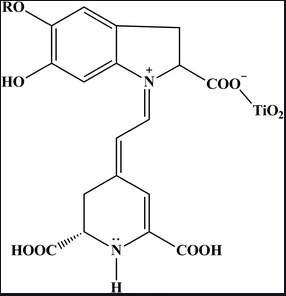
\includegraphics[width=0.25\textwidth]{Betalin_TiO2.png}
\caption{Betalin and TiO$_2$. \cite{betalinpicture}}
\label{fig:Betalin_TiO2} %use label to refer to it in later text.
\end{figure}

The second dye used in this experiment is made from black tea leaves with an efficiency of 0.20 \%. Research has been done between black and green tea leaves and it turned out that black tea was more efficient. The open-circuit voltage of green tea leaves amounts to 0.47V and of black tea leaves 0.55V \cite{blacktea} \cite{15naturaldyes}. The chosen tea leaves are of the brand 'Ceylon Cay', a popular Turkish tea, see fig.\ref{fig:cay}

\begin{figure}[h]
\centering
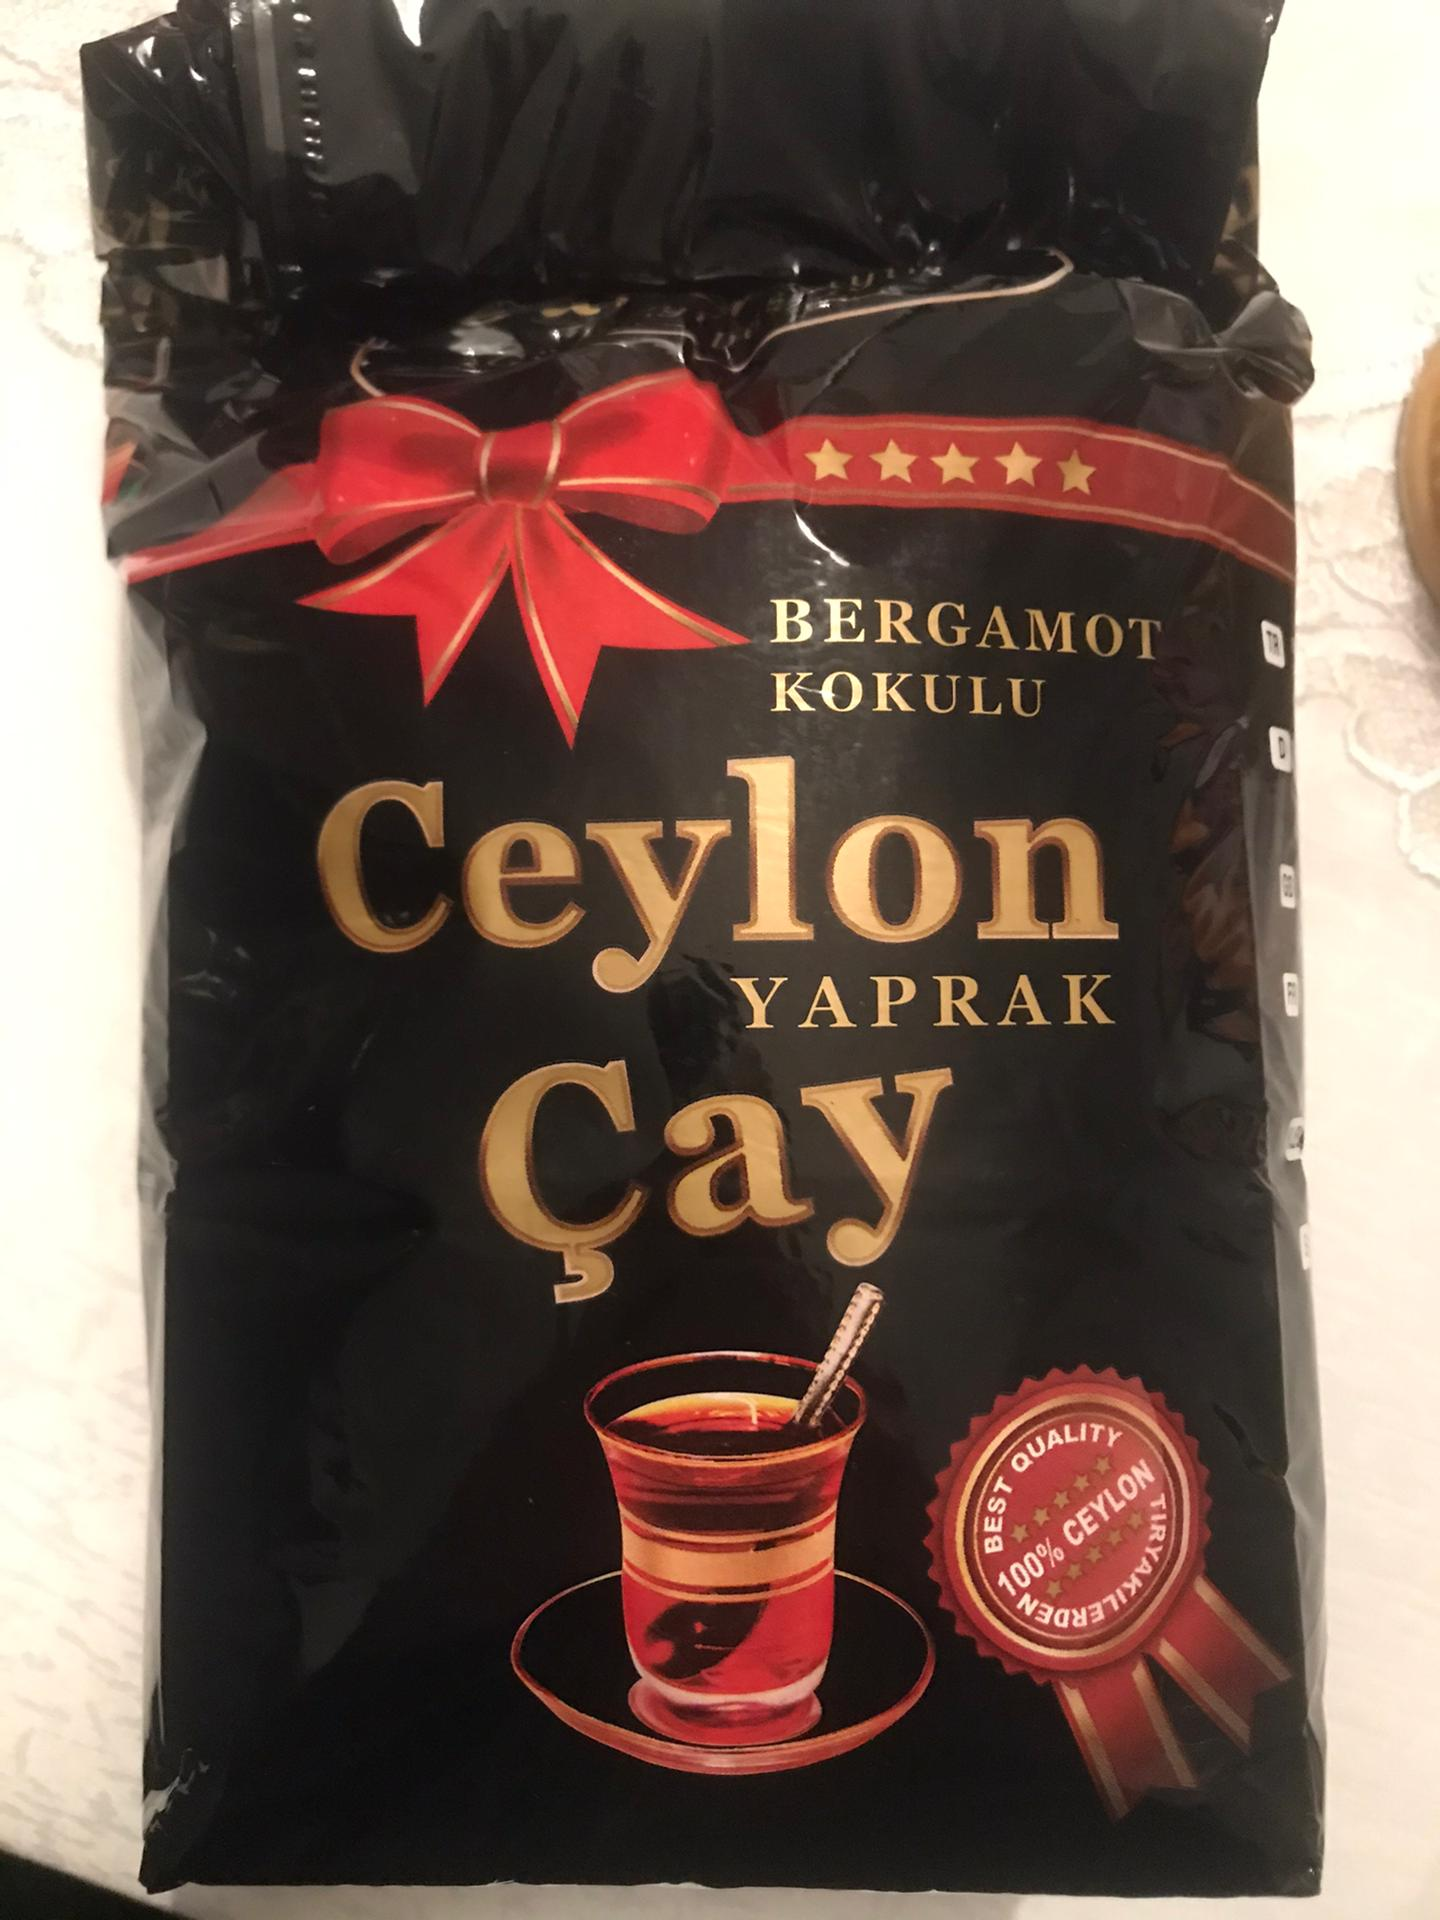
\includegraphics[width=0.25\textwidth]{cay.png}
\caption{Tea brand used in the experiment.}
\label{fig:cay} %use label to refer to it in later text.
\end{figure}

\subsection{Preparation of the dyes}
In this subsection the preparation of both dyes is discussed.\\
\subsubsection{Beetroot}
For the first dye beetroot was used. This dye was prepared two days before the actual lab to save some time during the experiment. The dye was kept at room temperature in a sealed container as seen in fig. \ref{fig:dyepreparationbeet}. A total of 0.48 kilograms beetroot was chopped roughly with a kitchen knife and then mixed together with roughly 300 ml tap water. After the mixture was finely chopped by the mixer the rough bits of beet were separated using a sieve, leaving dark beetroot juice. The beetroot juice was then filtered another time using a coffee filter. The final result was the dye used for the first solar cell.

\begin{figure}[h]
\centering
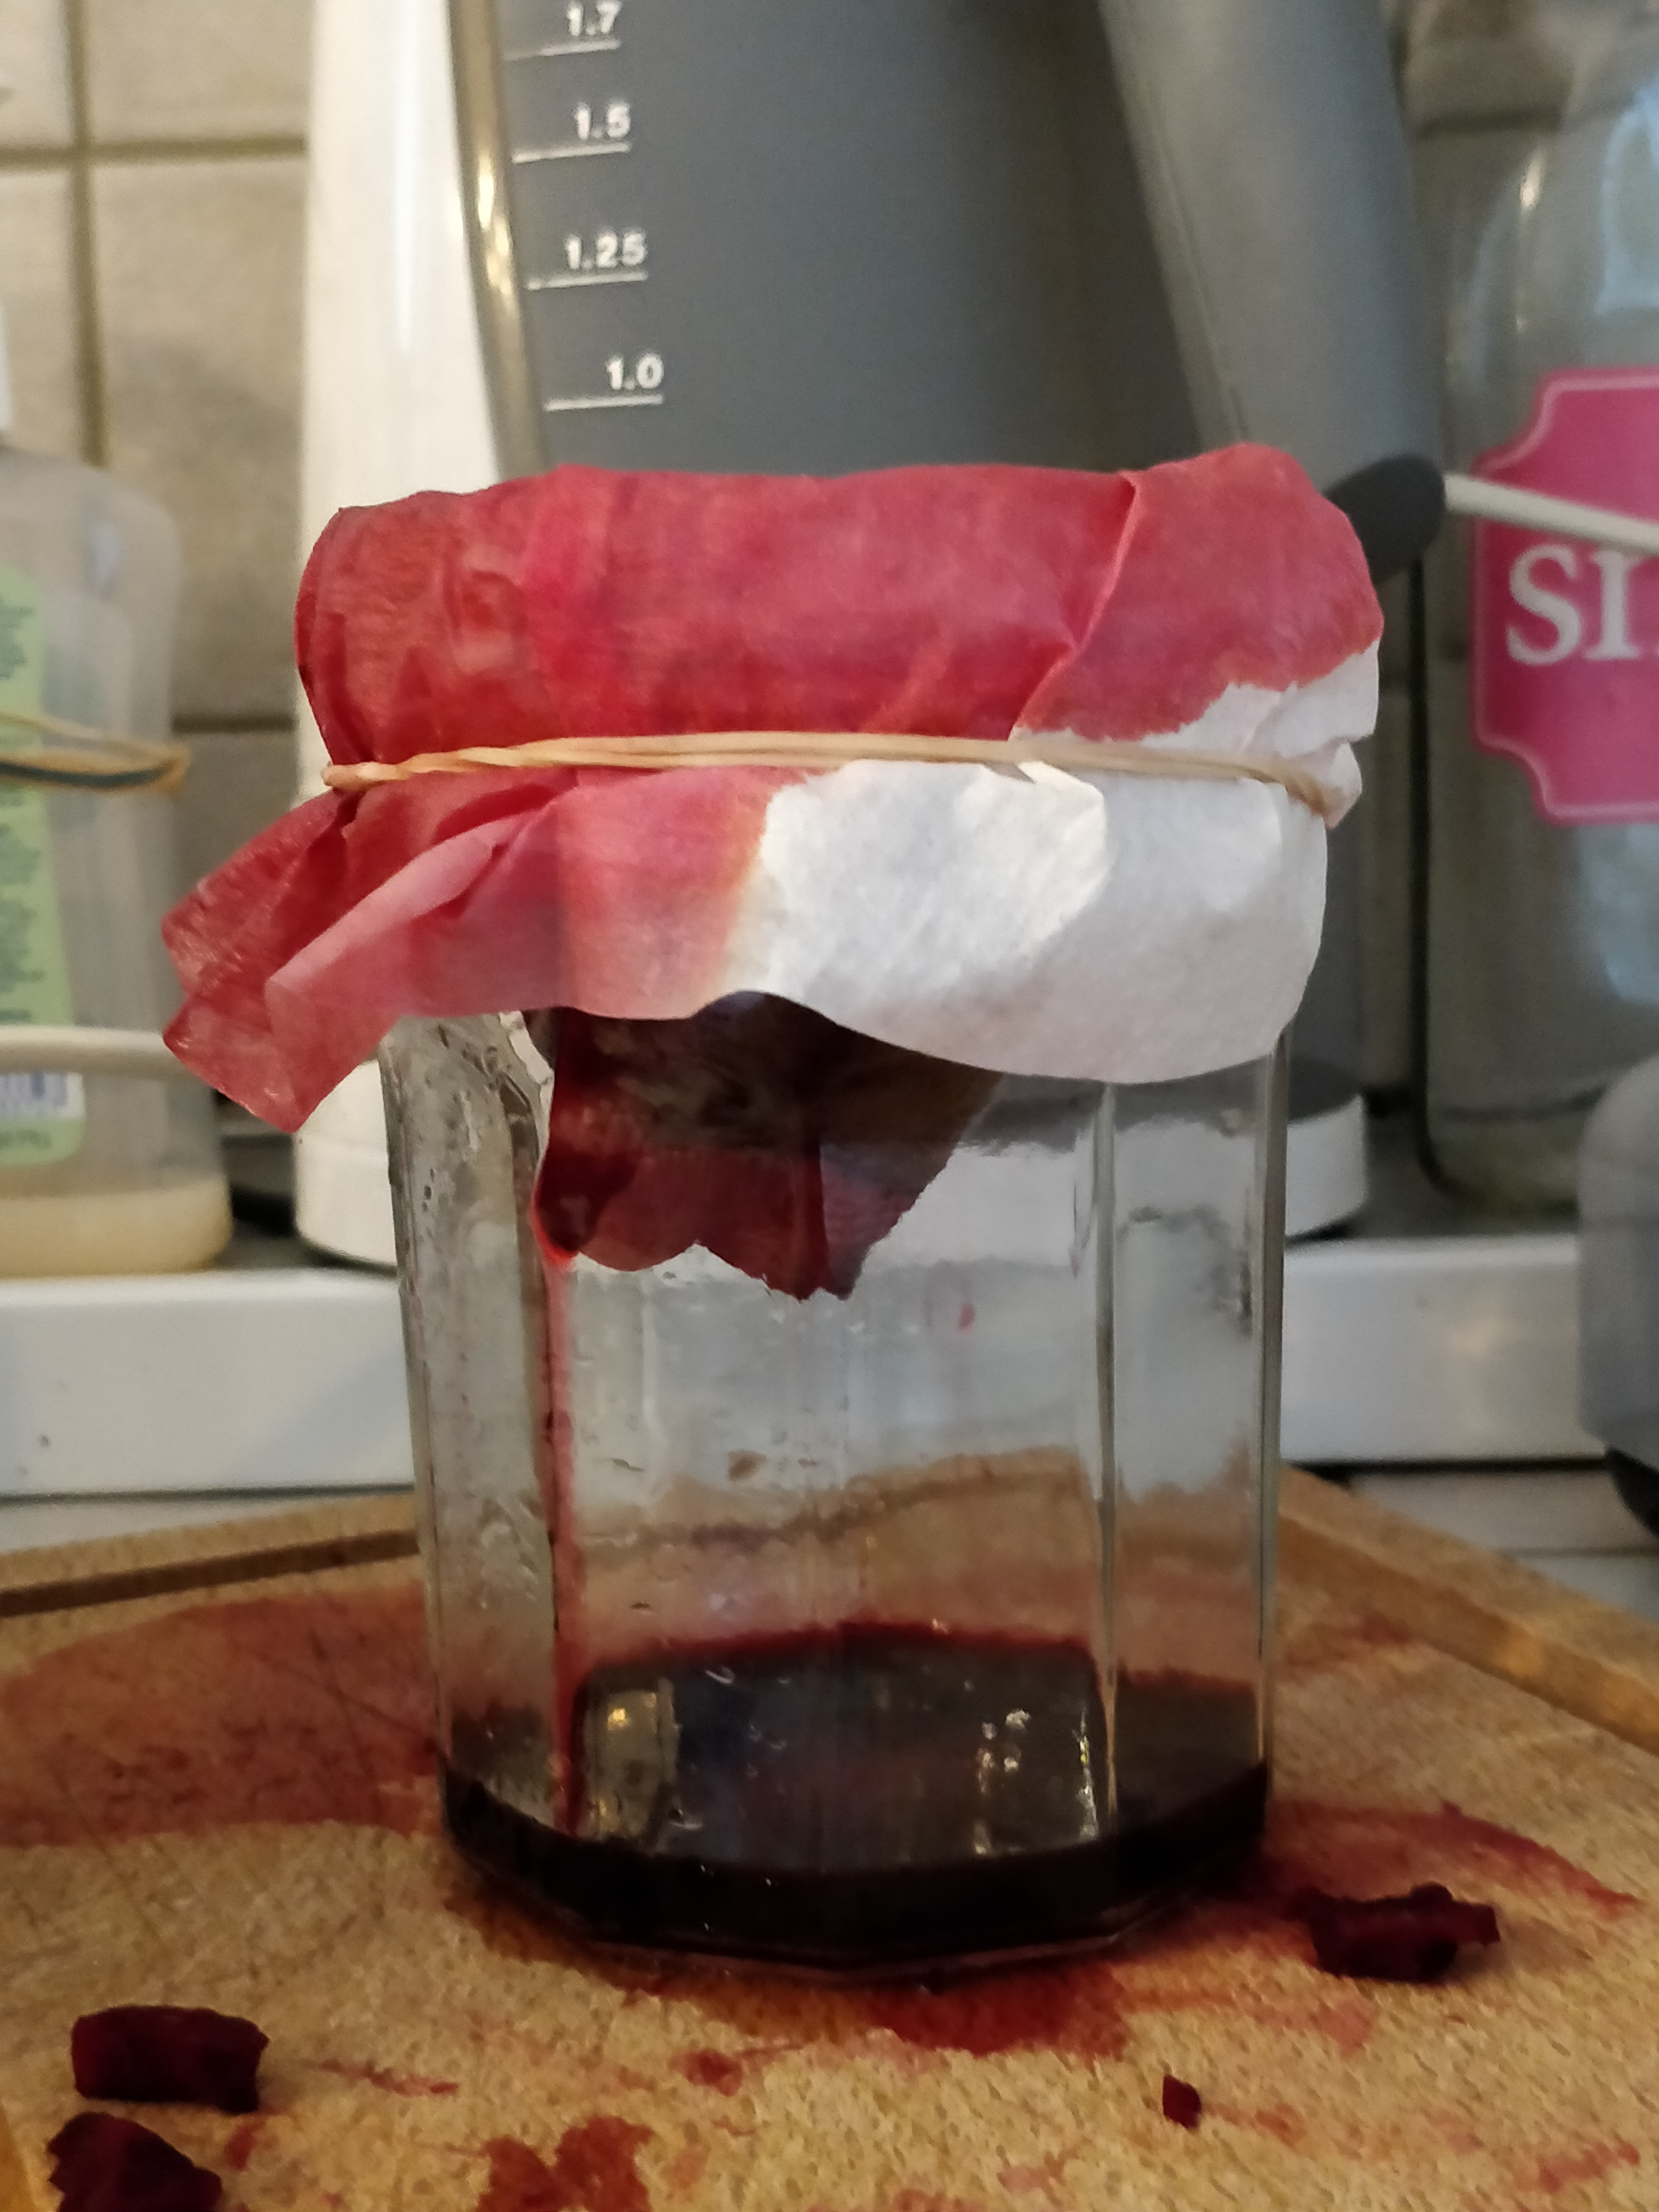
\includegraphics[width=0.25\textwidth]{DyePreparationBeet.jpg}
\caption{Filtering the dye.}
\label{fig:dyepreparationbeet} %use label to refer to it in later text.
\end{figure}

\subsubsection{Black tea}
The second dye used is black tea. For making this dye, black tea leaves, boiling water, a cup and a spoon where required. Black tea leaves are available virtually everywhere in general convenience stores and supermarkets. The tea leaves that are used in this experiment are a brand of Turkish black tea leaves. The black tea leaves in the container can be seen in fig. \ref{fig:black tea in cup}. 

\begin{figure}[h]
\centering
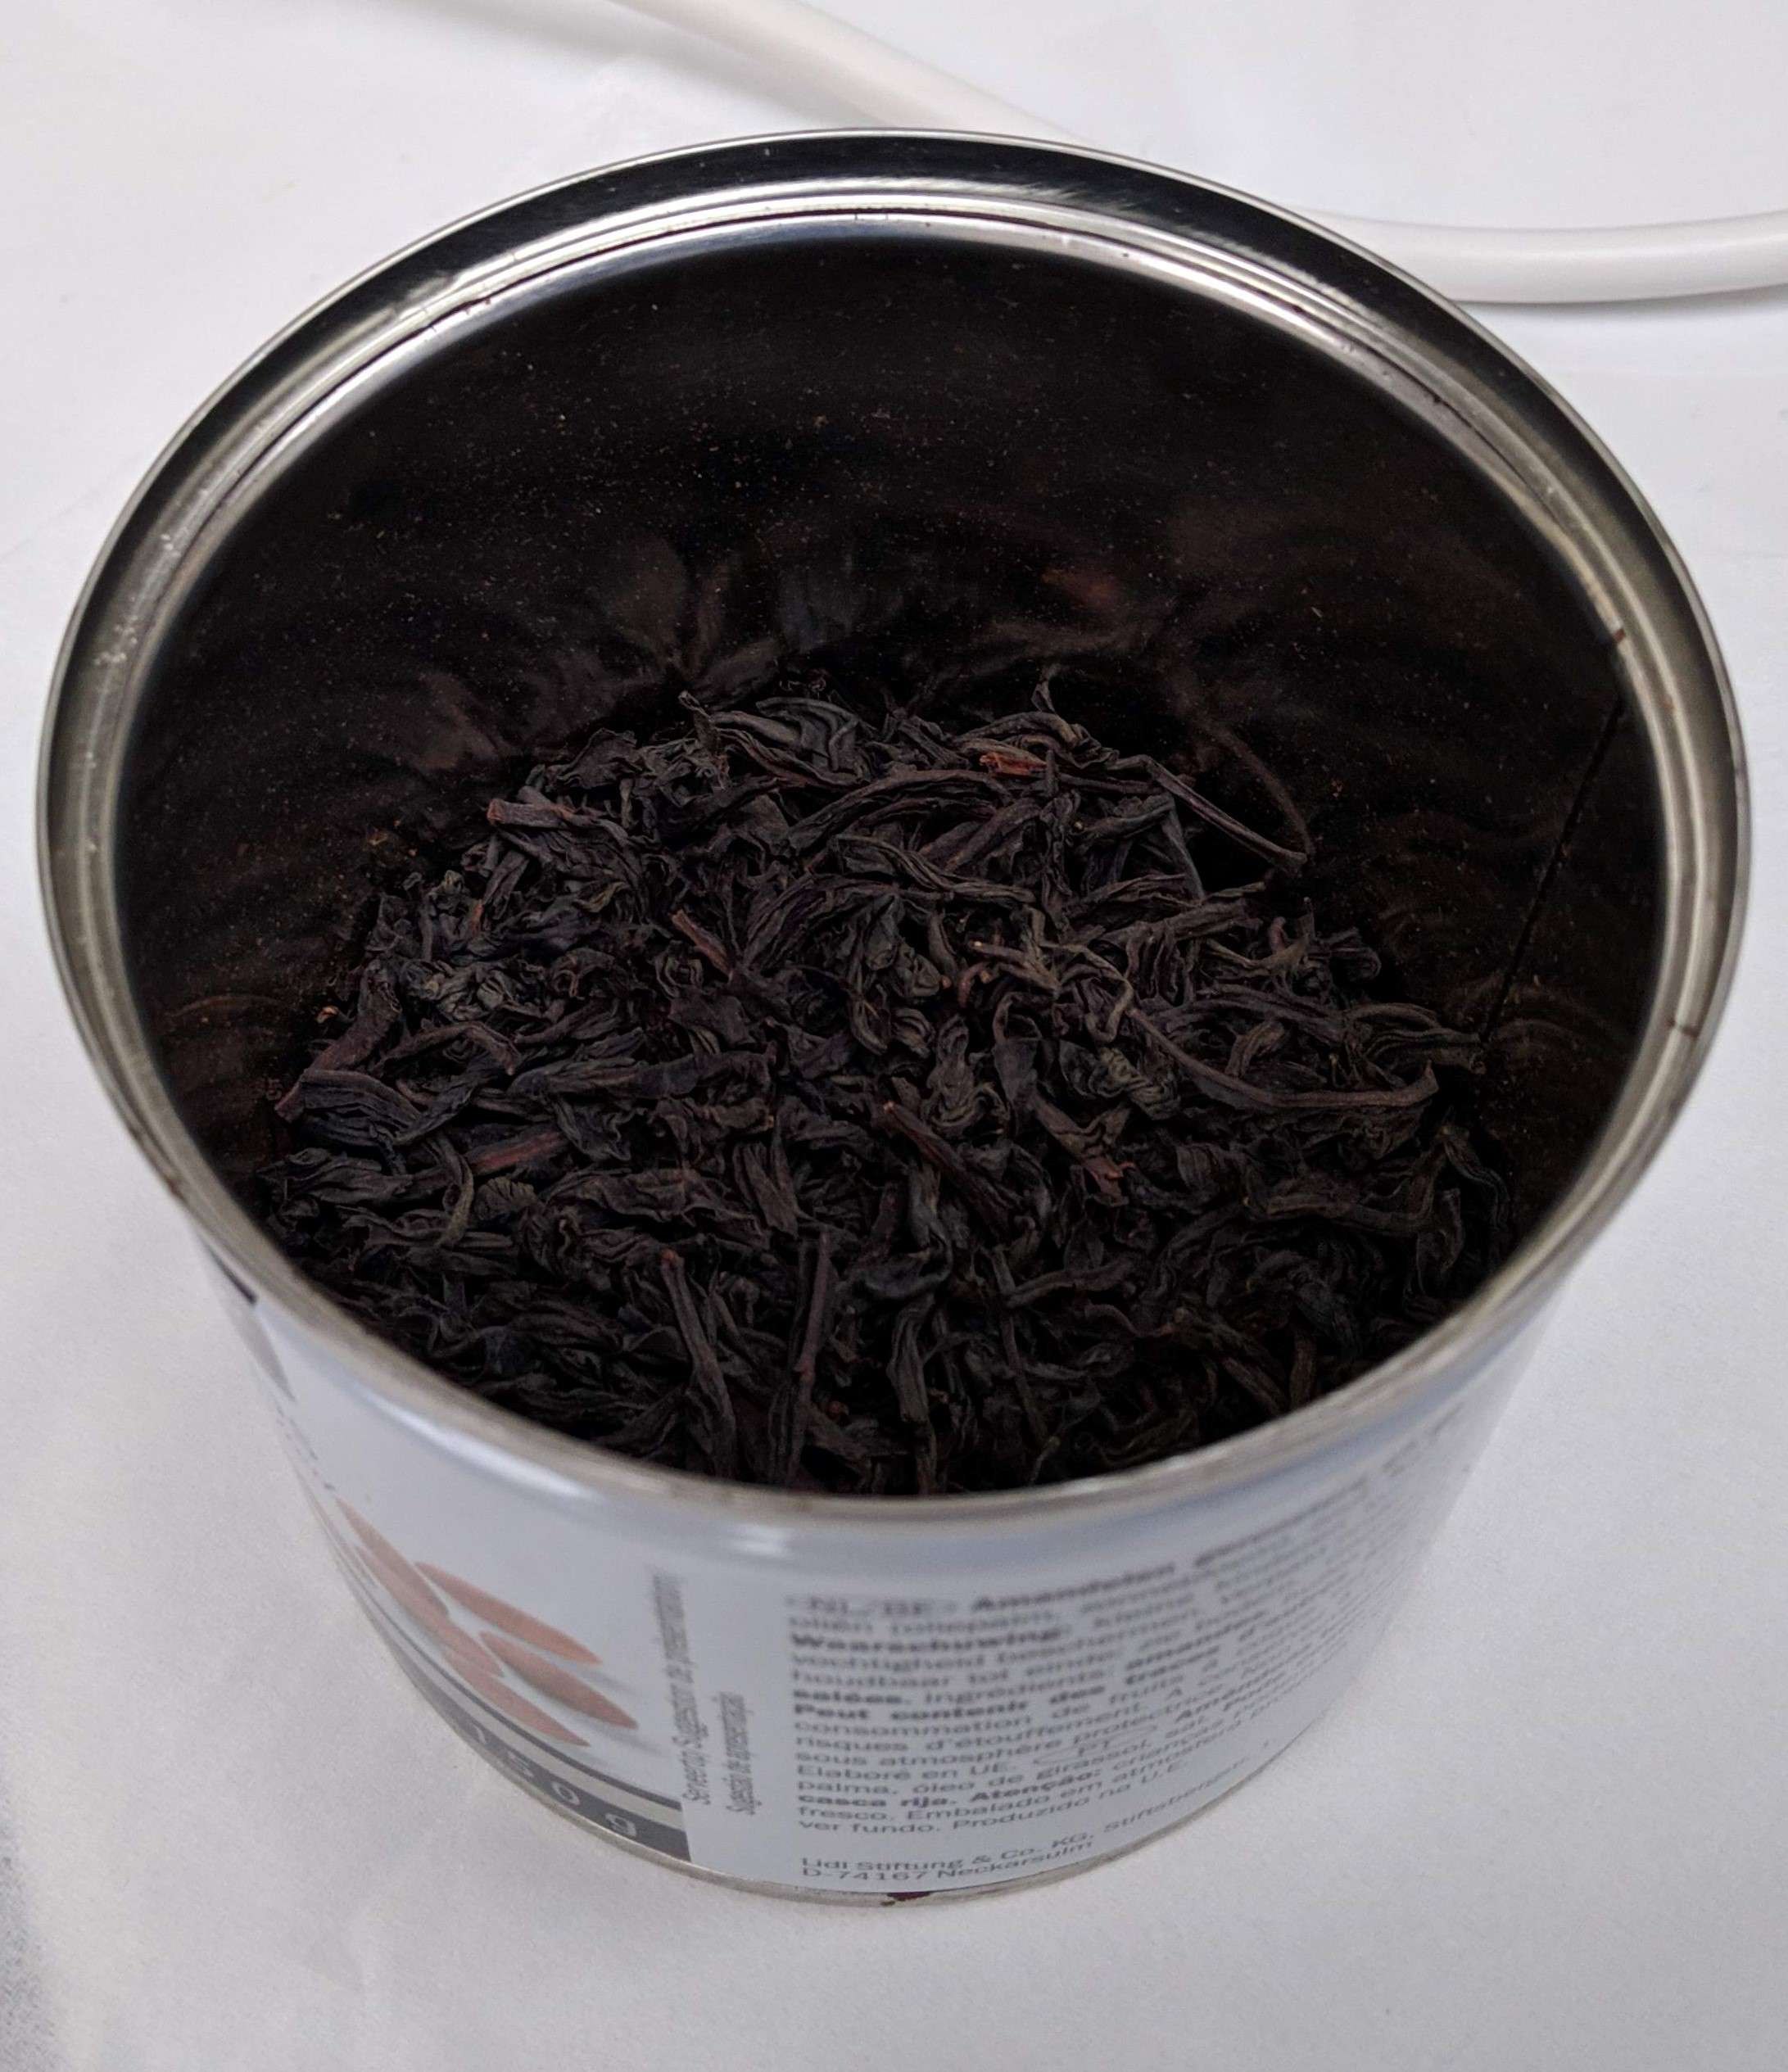
\includegraphics[width=0.25\textwidth]{15BlackTea1.jpg}
\caption{Black tea leaves in a cup.}
\label{fig:black tea in cup} %use label to refer to it in later text.
\end{figure}

With the black tea leaves in the container, the boiling water can be added. As can be seen in  fig. \ref{fig:add hot water}. In order to get the tea as strong as possible, the amount of leaves was rather high and at regular intervals, the heterogeneous mixture was stirred. 

\begin{figure}[H]
\centering
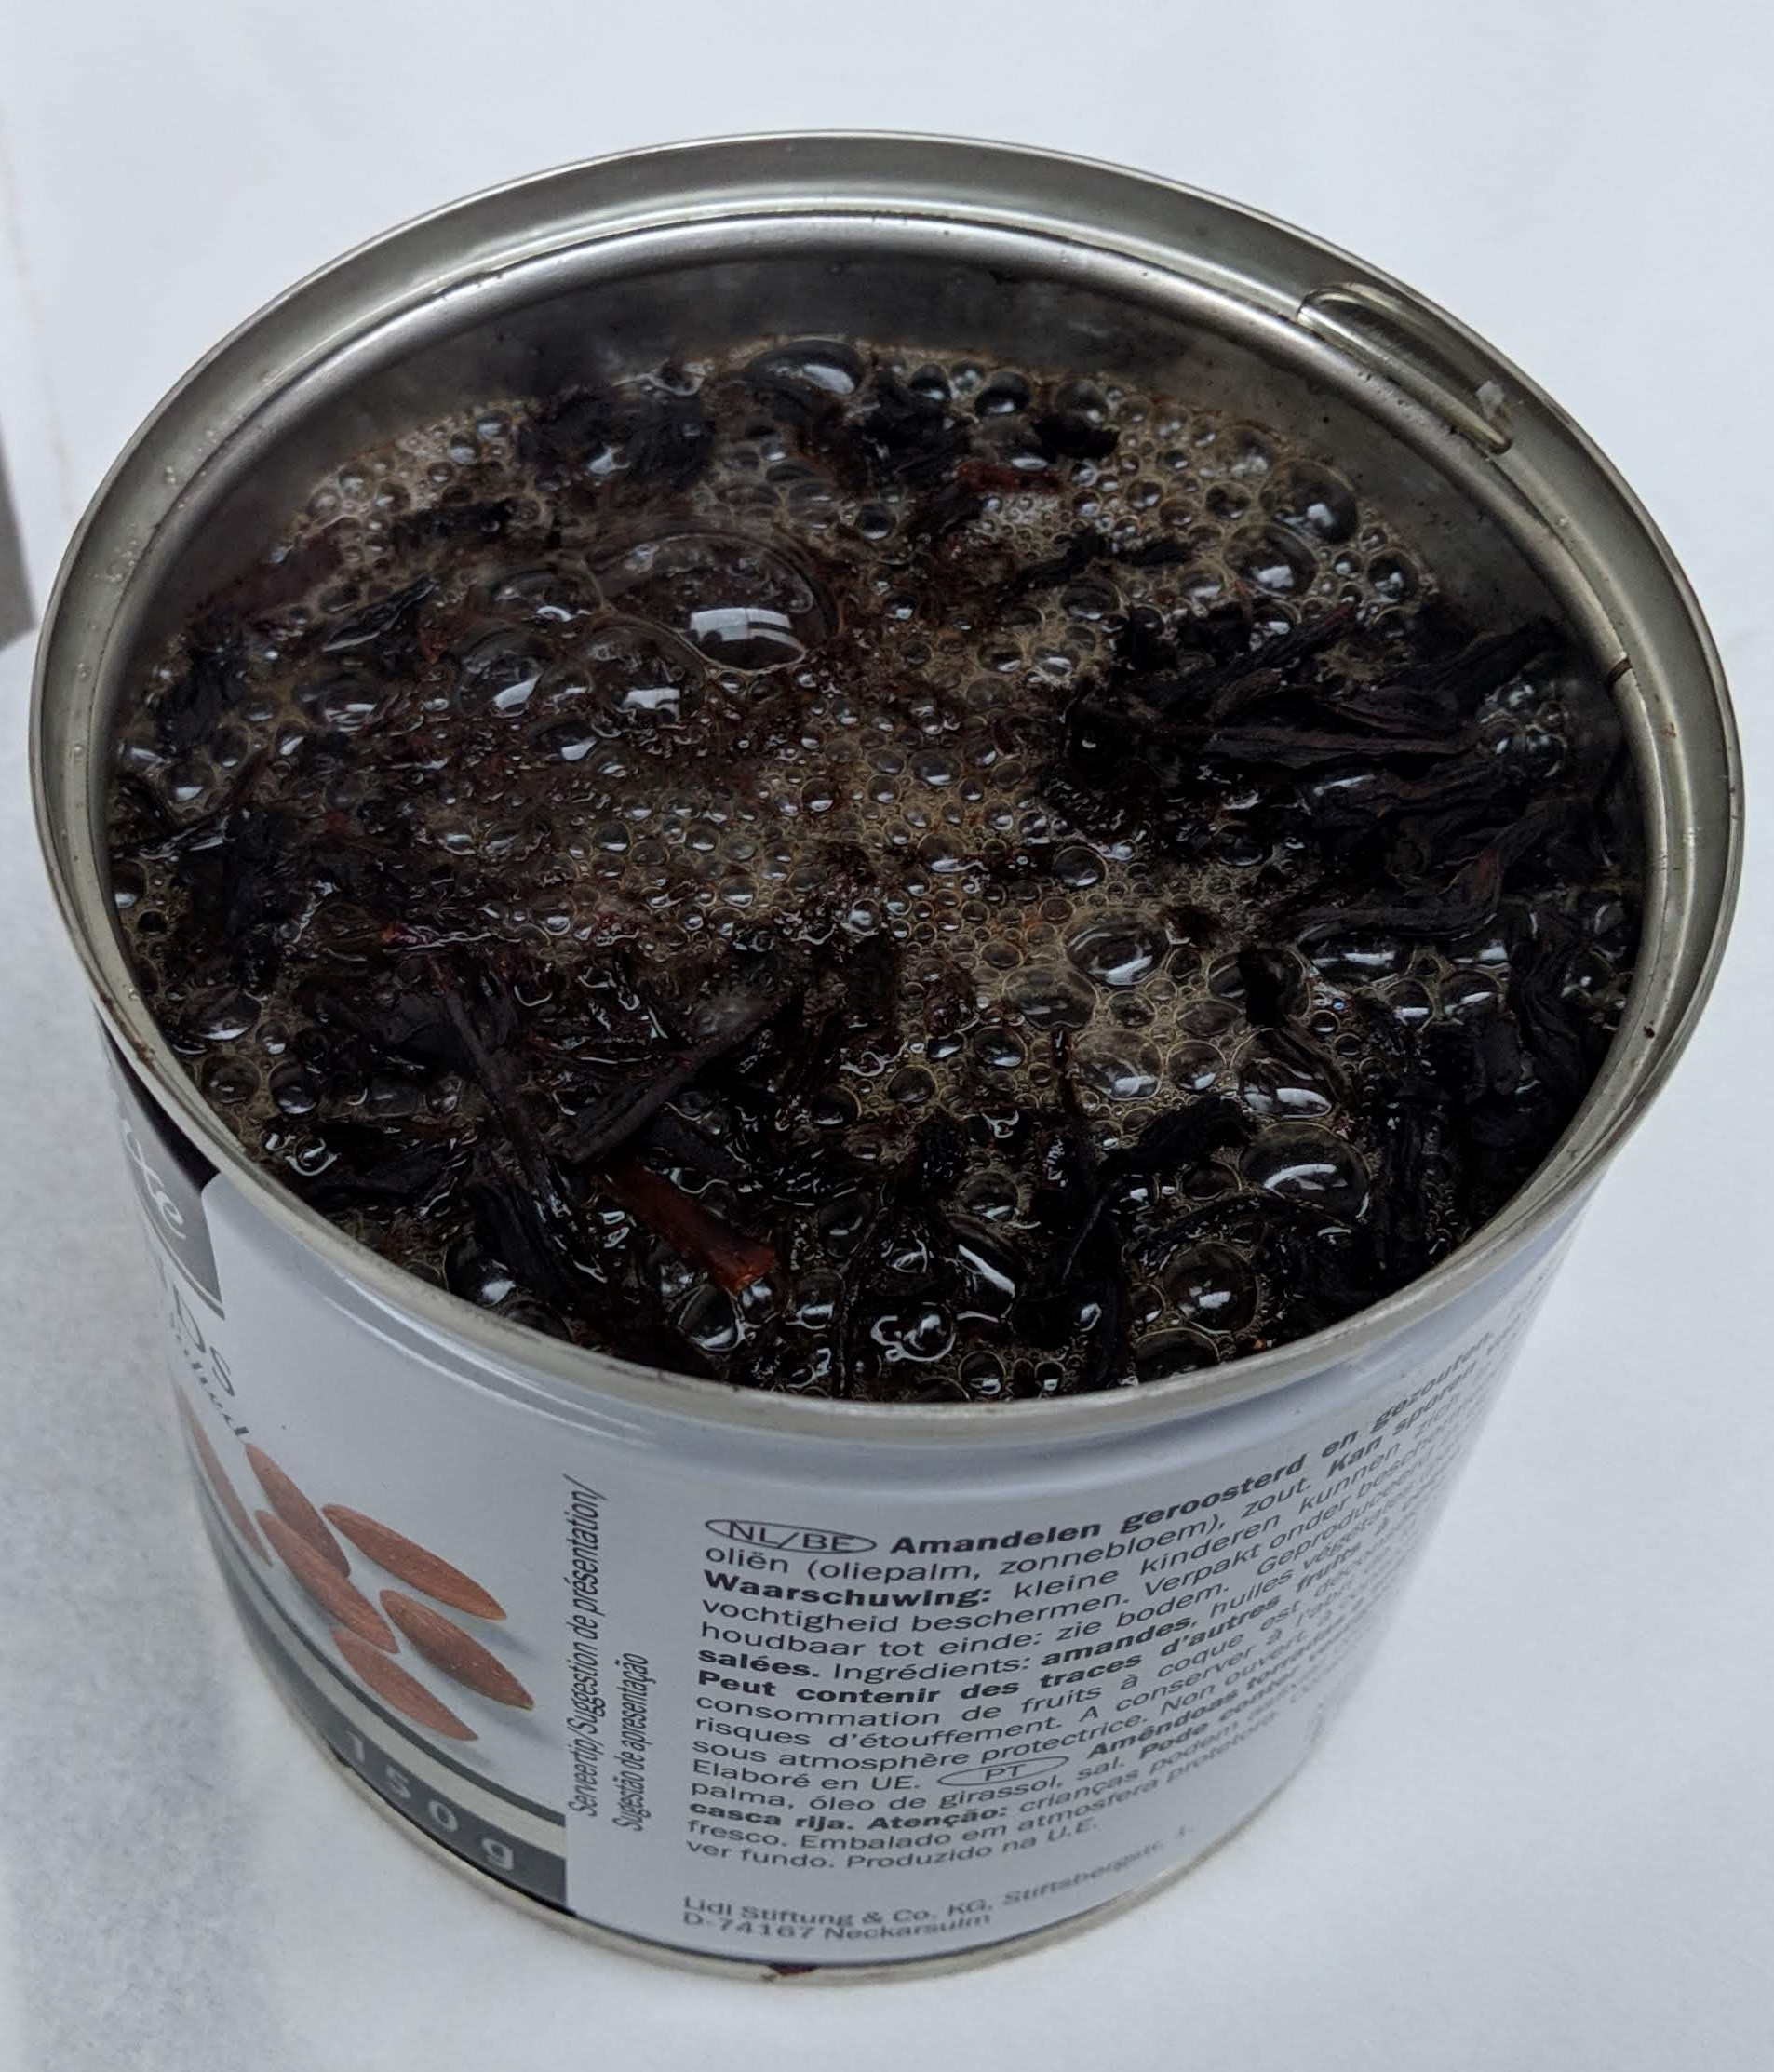
\includegraphics[width=0.25\textwidth]{16BlackTea2.jpg}
\caption{Black tea leaves with boiling water.}
\label{fig:add hot water} %use label to refer to it in later text.
\end{figure}

When the tea cools down to a manageable temperature the tea leaves can be filtered out. The remaining liquid (strong black tea) is used as the dye for the second solar cell.


\subsection{Preparation of the glass}
First step was to take the glass plates and measure the conductive side with a multimeter. After verifying the conductive side, it was placed upwards on a piece of paper.

\subsubsection{Preparation of anode}
Take the glasses and used a pencil to apply graphite to the conductive side. For each cell, there has to be one anode side. In this case, three cells where made. Therefore, three anodes have to be made.

\begin{figure}[H]
\centering
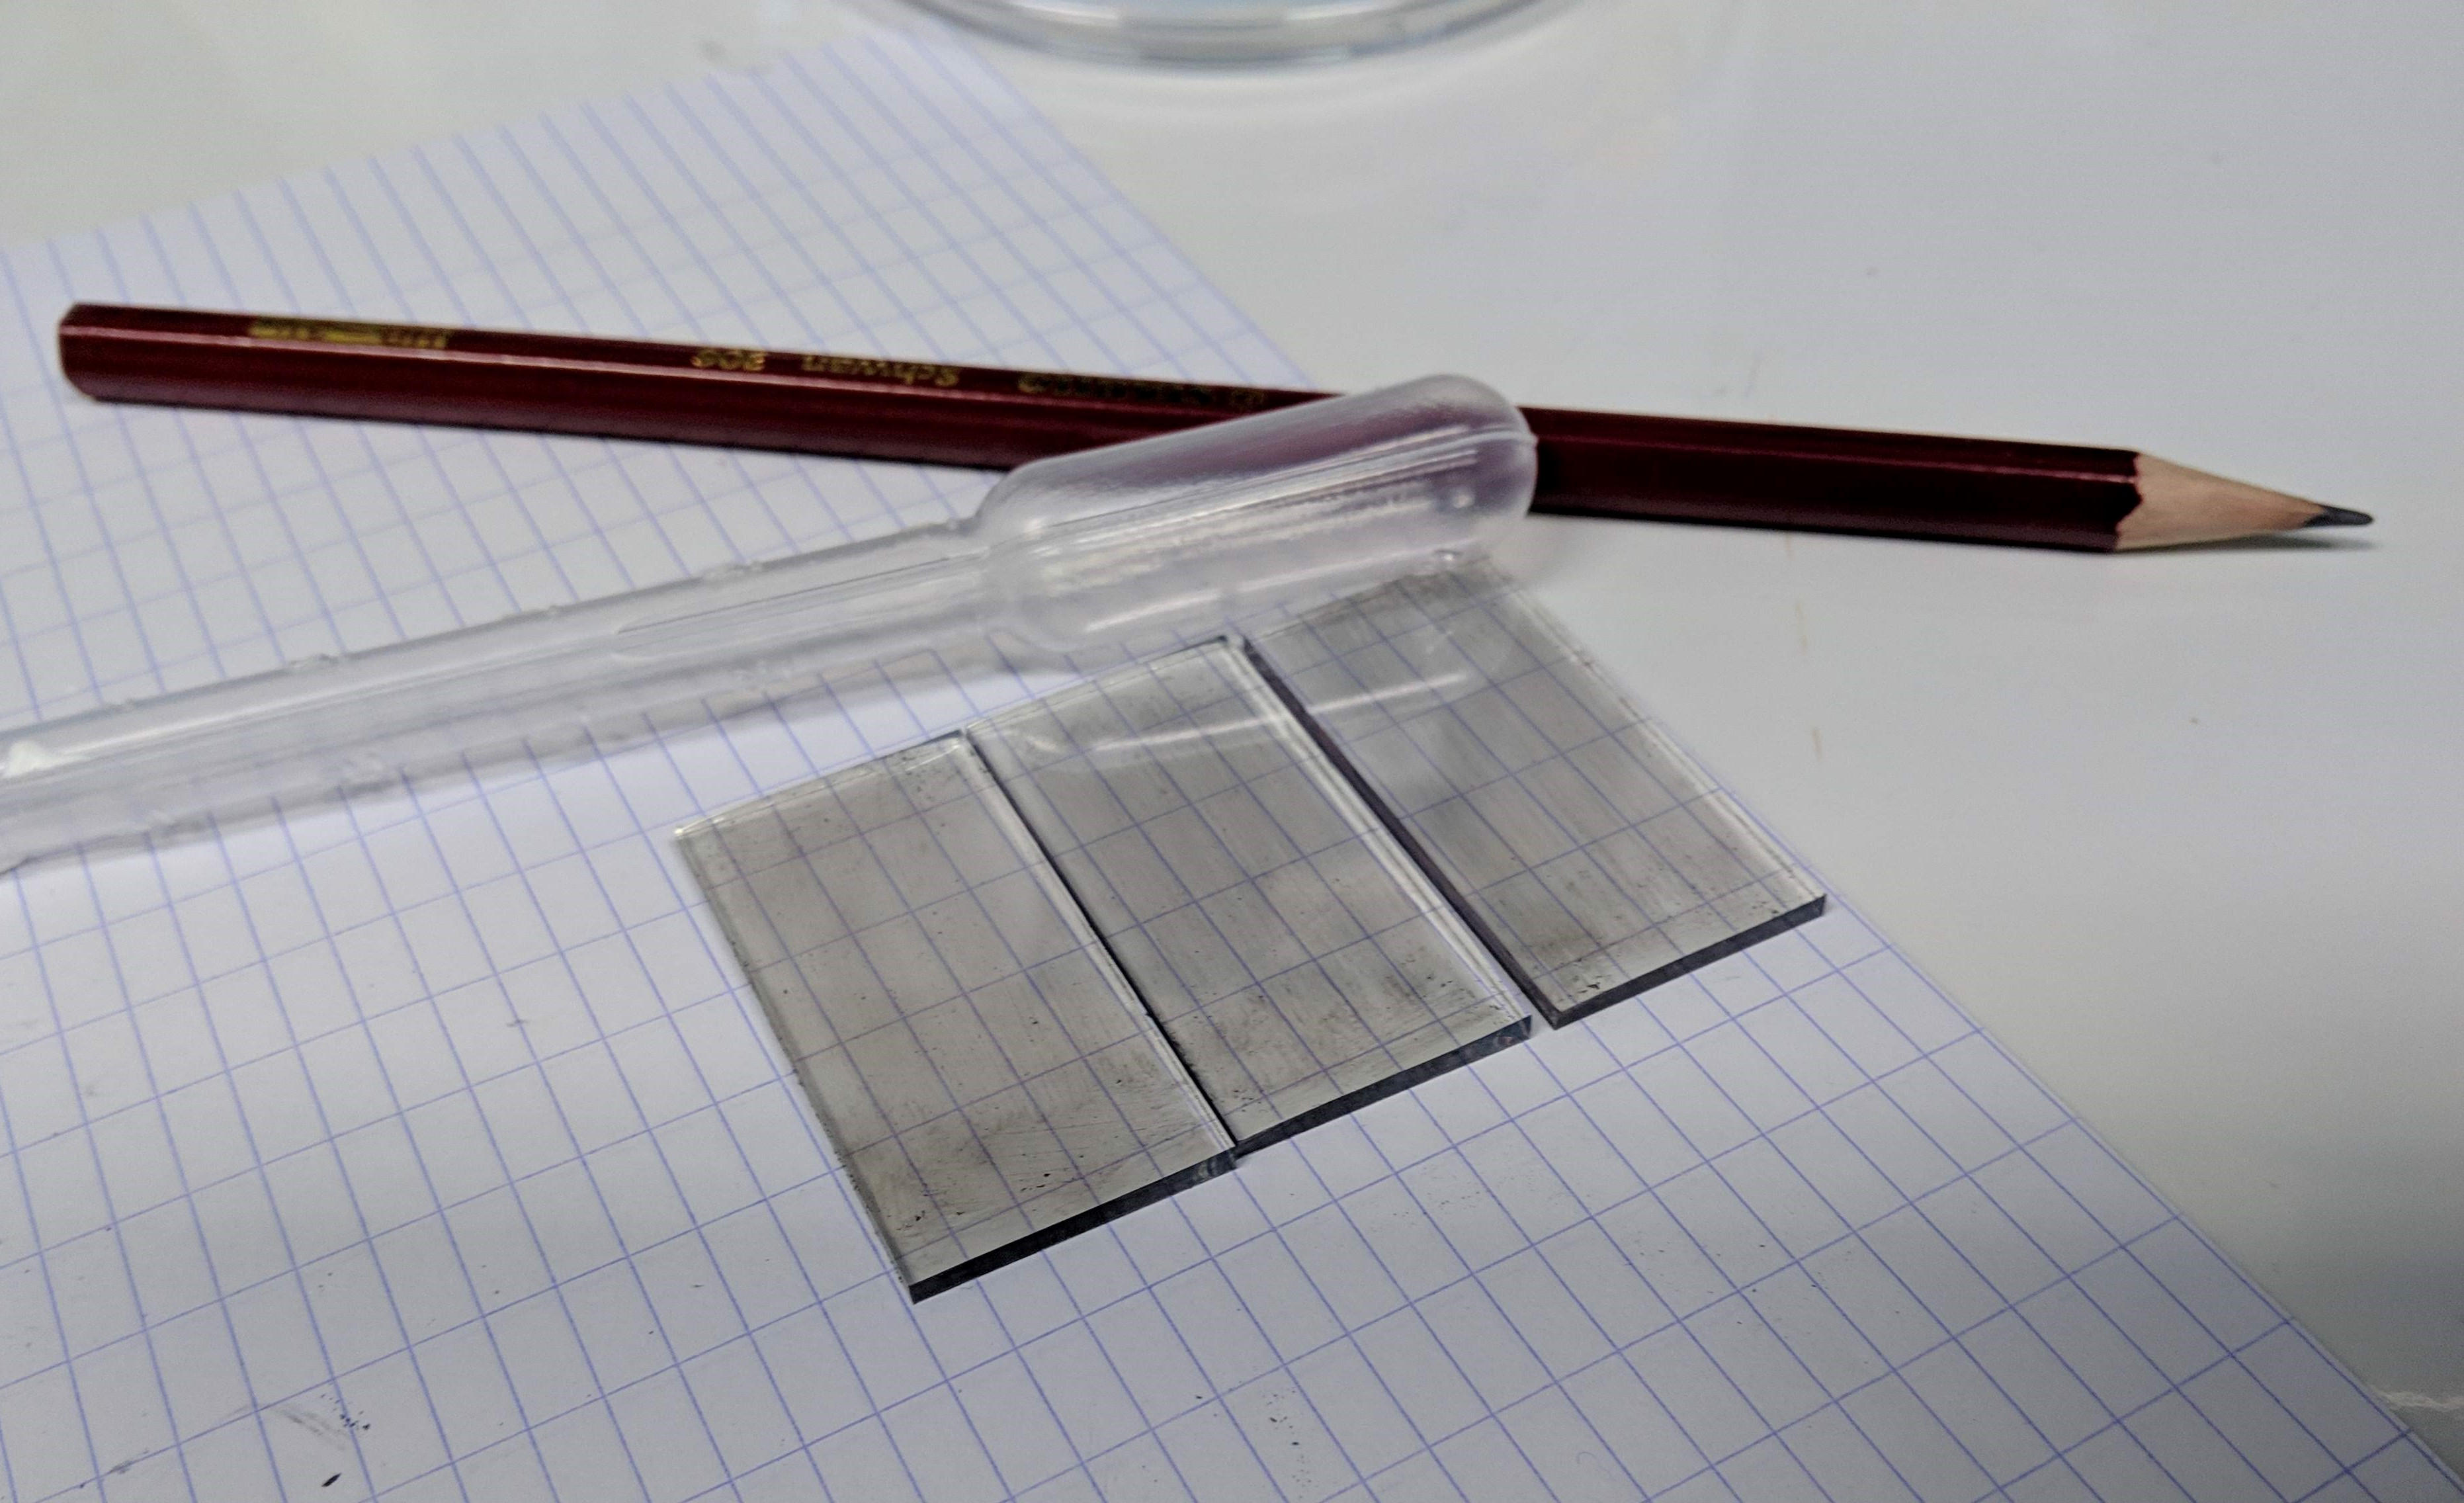
\includegraphics[width=8.0cm]{4GraphiteLayer.jpg}
\caption{Applying graphite to the anode.}
\label{fig:graphitelayer} %use label to refer to it in later text
\end{figure}
\subsubsection{Preparation of cathode}
The edges of the cathode were taped using scotch tape. After this 1 droplet of TiO$_2$ paste was applied to the cathode. The layer should be thinned out as much as possible using a glass plate. After a satisfactory thickness is achieved, the scotch tape can be removed carefully. The cathode can then be transferred onto a piece of folded aluminium foil and heated using the hot plate as seen in figure \ref{fig:heatingti2o}.

\begin{figure}[H]
\centering
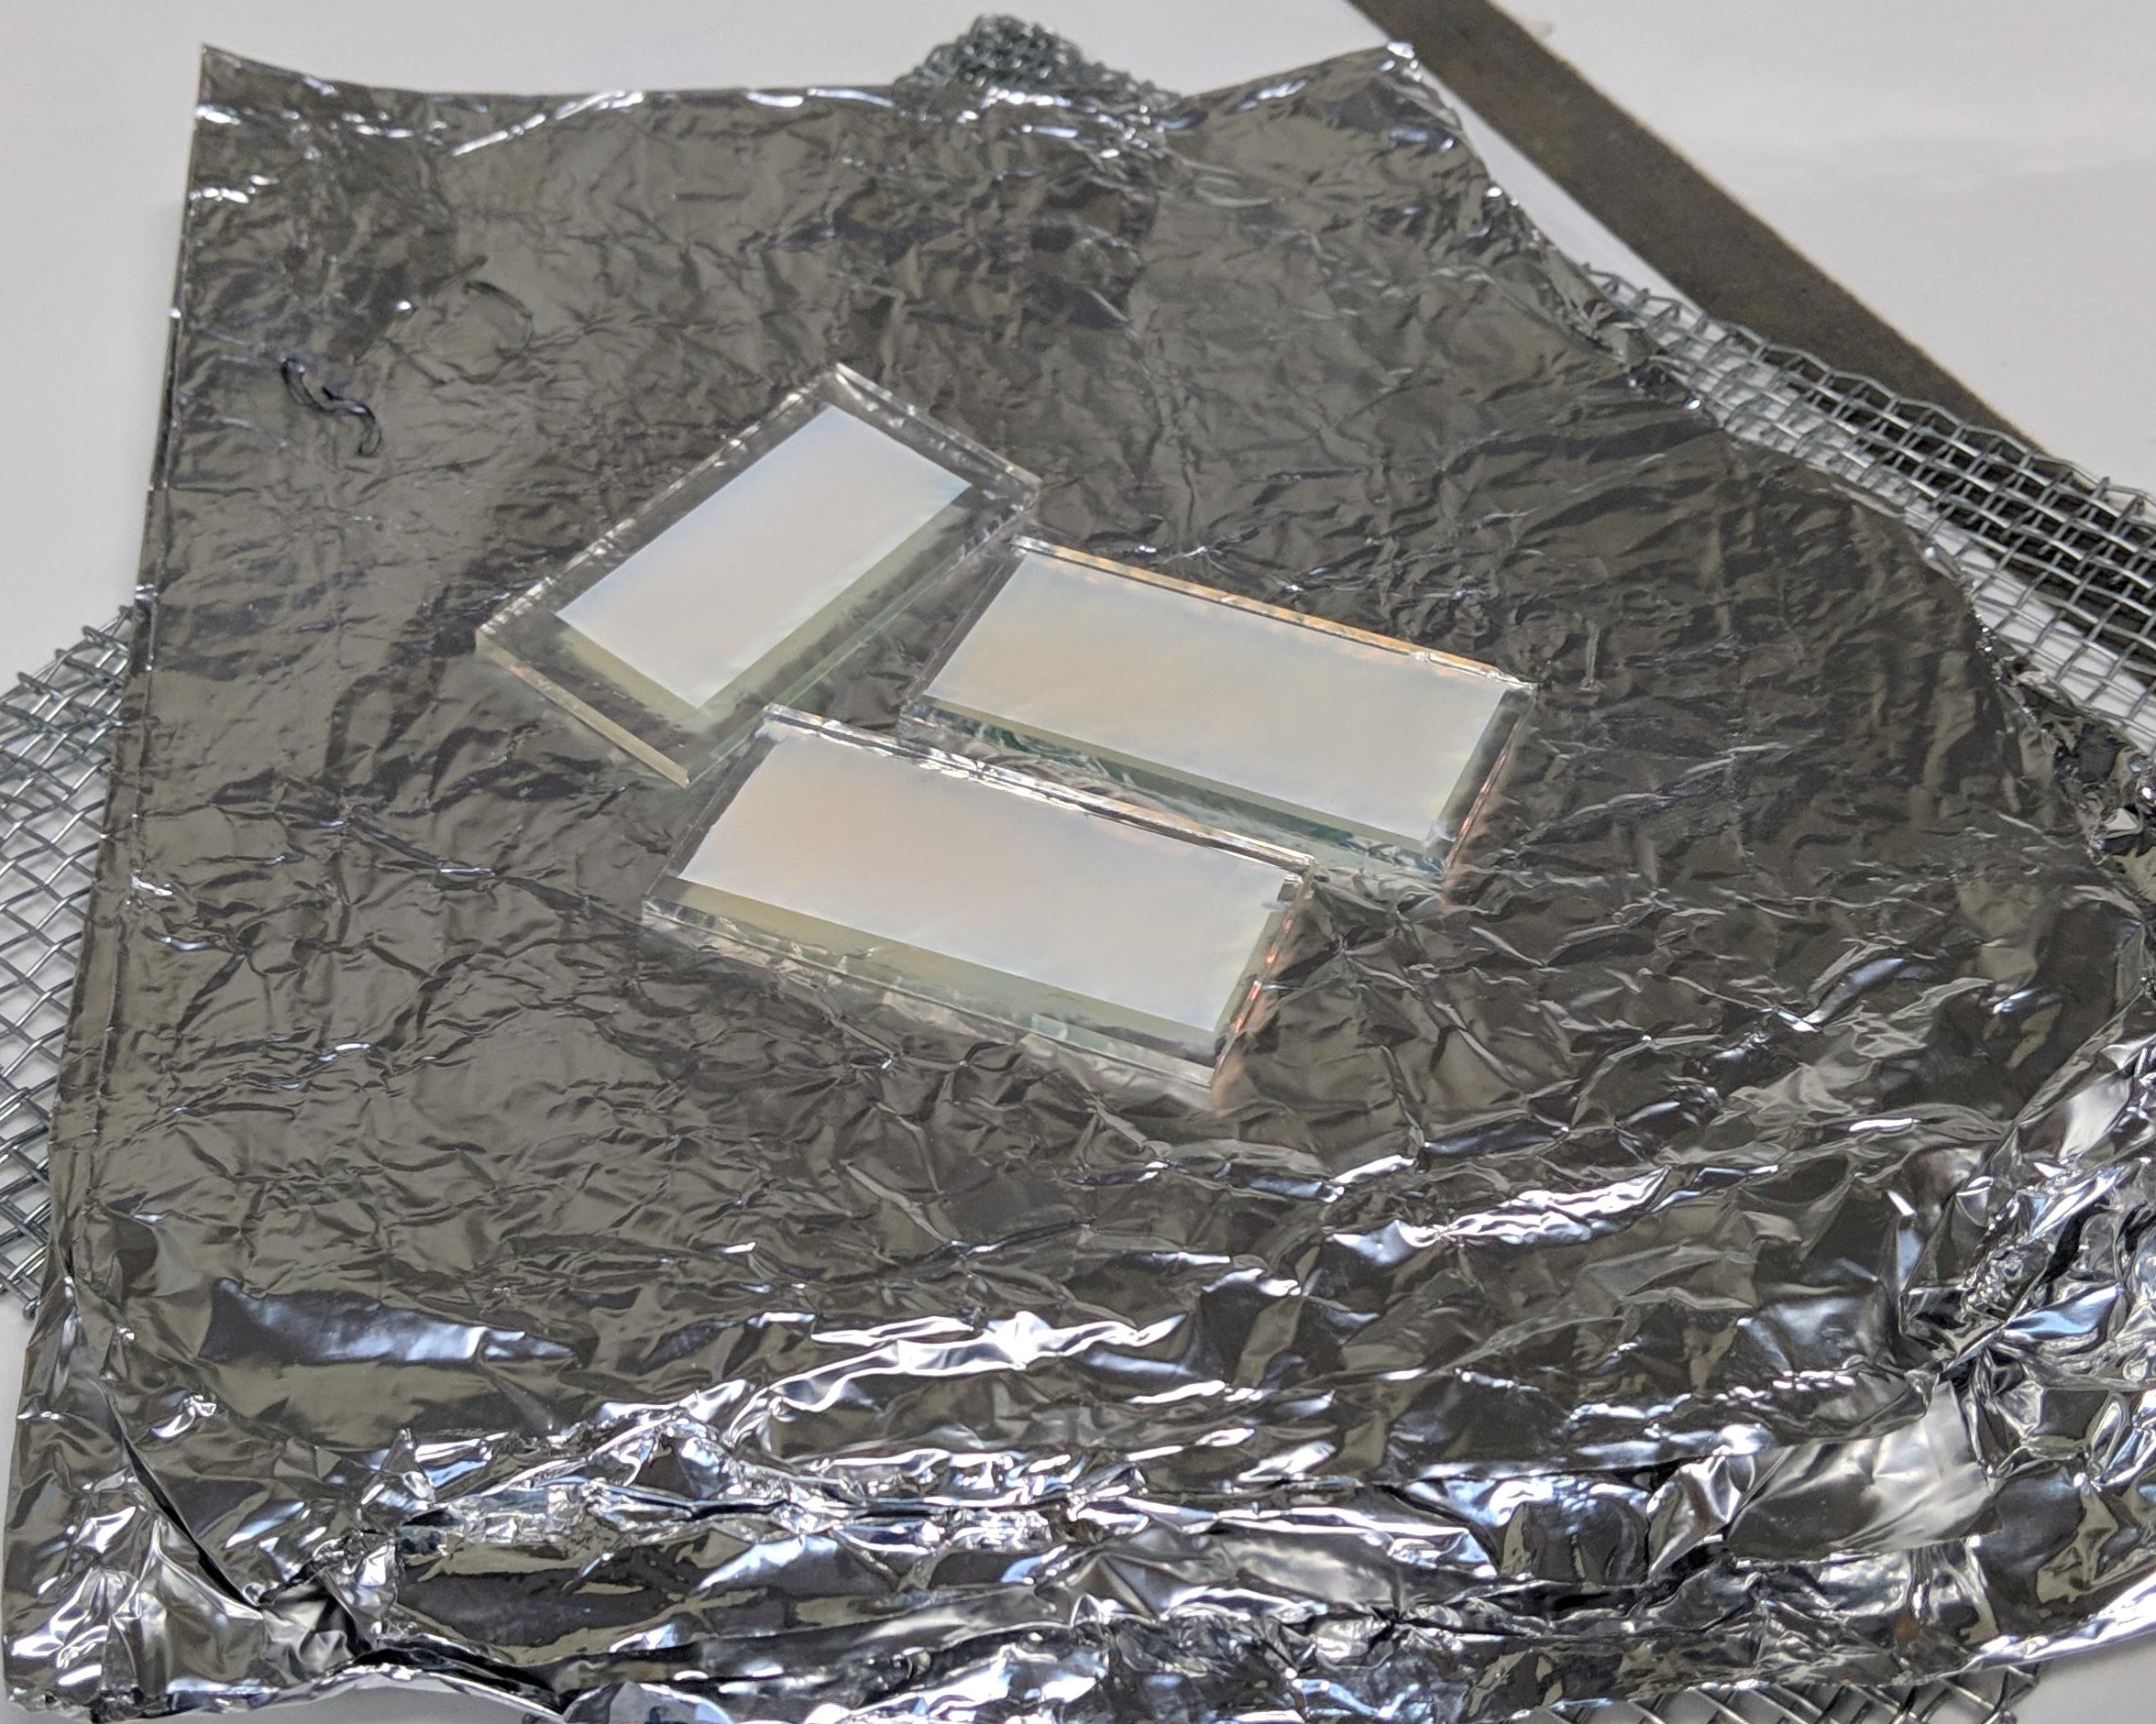
\includegraphics[width=0.35\textwidth]{2HeatedTiO.jpg}
\caption{Heating the TiO$_2$ paste.}
\label{fig:heatingti2o} %use label to refer to it in later text
\end{figure}

Each cathode can then be put into a petri dish to apply the beetroot and black tea dye as seen in figure \ref{fig:dyesetup}. The cathode for the beetroot dye was first submerged for ten minutes and then rinsed with tap water.However, the dye was not fully attached to the TiO$_2$ paste, as it rinsed right off, so we decided to submerge it for another twenty minutes, totalling 30 minutes for the red dye. Also, see Research of the dyes \ref{ResearchDyes}, betalin is a water-soluble pigment. Therefore, the rinsing washed away the dye.\\

The black tea dye successfully attached to the TiO$_2$, but to keep timings consistent the glass plate was also submerged for 30 minutes in the black tea dye.

\begin{figure}[H]
\centering
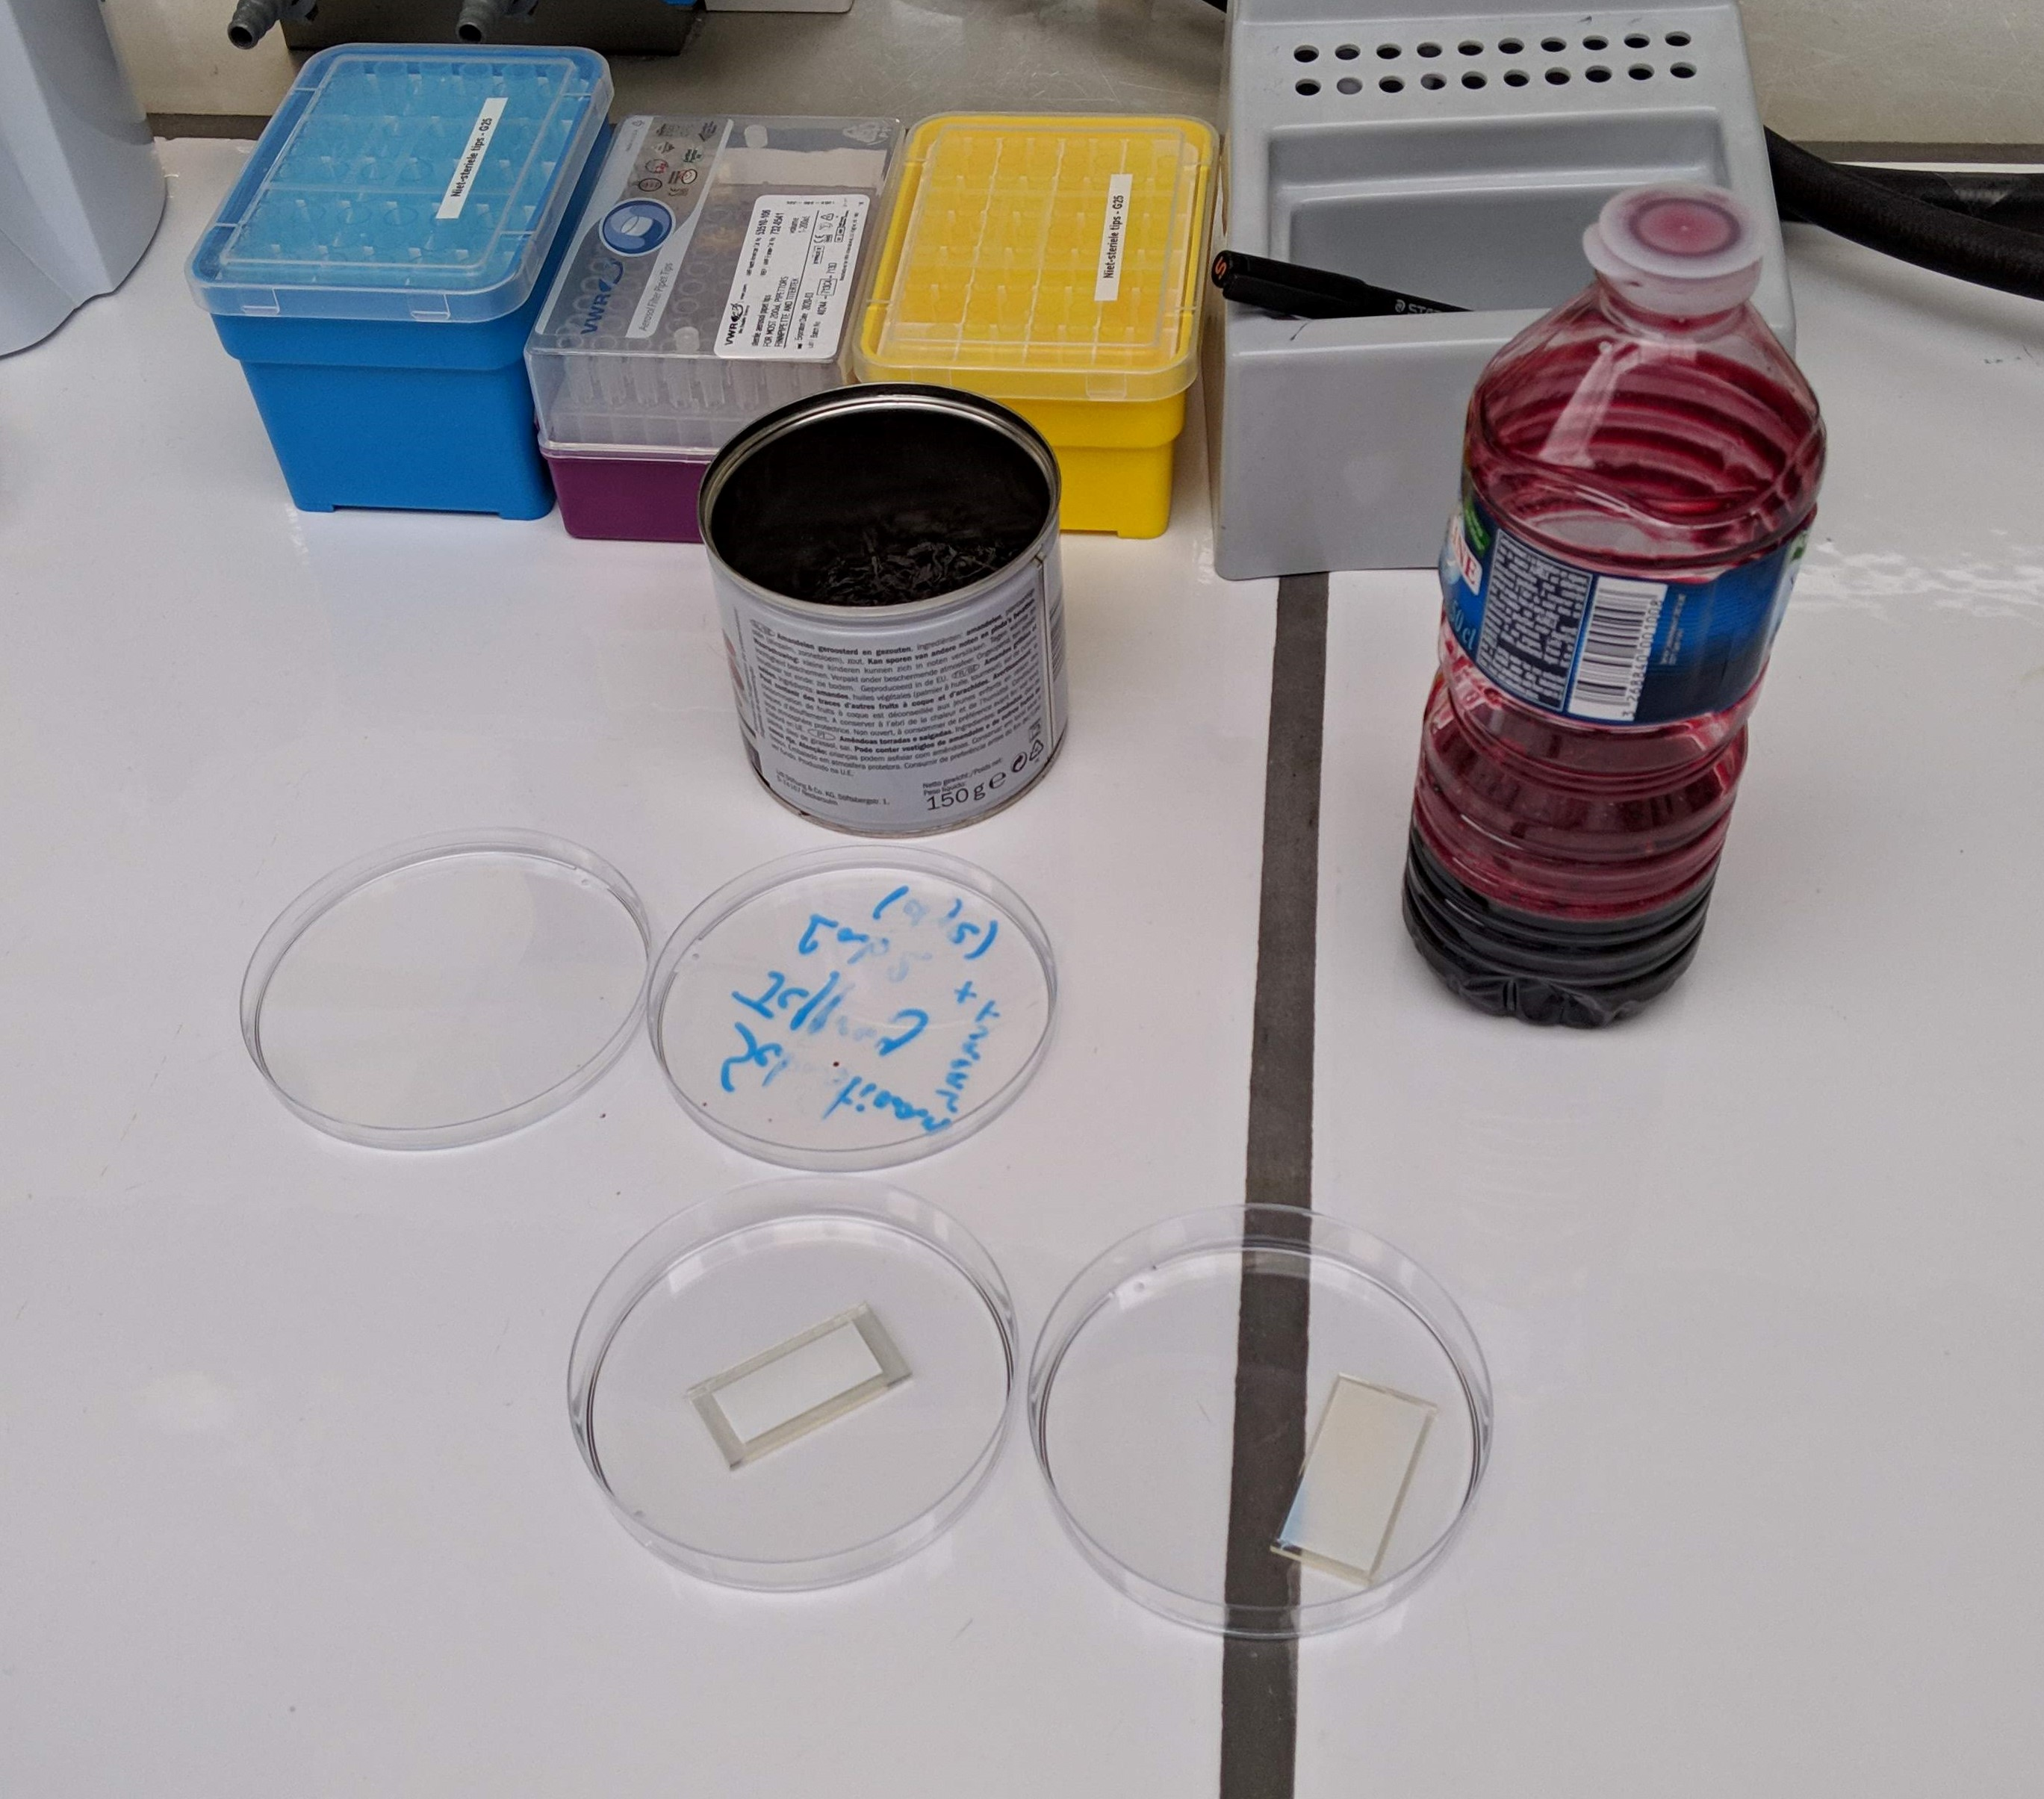
\includegraphics[width=0.35\textwidth]{12StartLab2.jpg}
\caption{Dye set up for cathode (Left: Black tea, Right: beetroot).}
\label{fig:dyesetup} %use label to refer to it in later text
\end{figure}

\subsubsection{Assembling the cells}
To assemble the cells, take the anode and cathode from the paper. Add one single droplet of electrolyte to the cathode. Next, clip together both conductive sides facing inwards with a paper clip bent as mentioned in the introduction \ref{intro}.
The excess electrolyte can be wiped away with a paper tissue to taking a measurement an easy process. A final result from the first solar cell made with Hibiscus dye can be seen in figure \ref{fig:resultsolarcell}.

\begin{figure}[H]
\centering
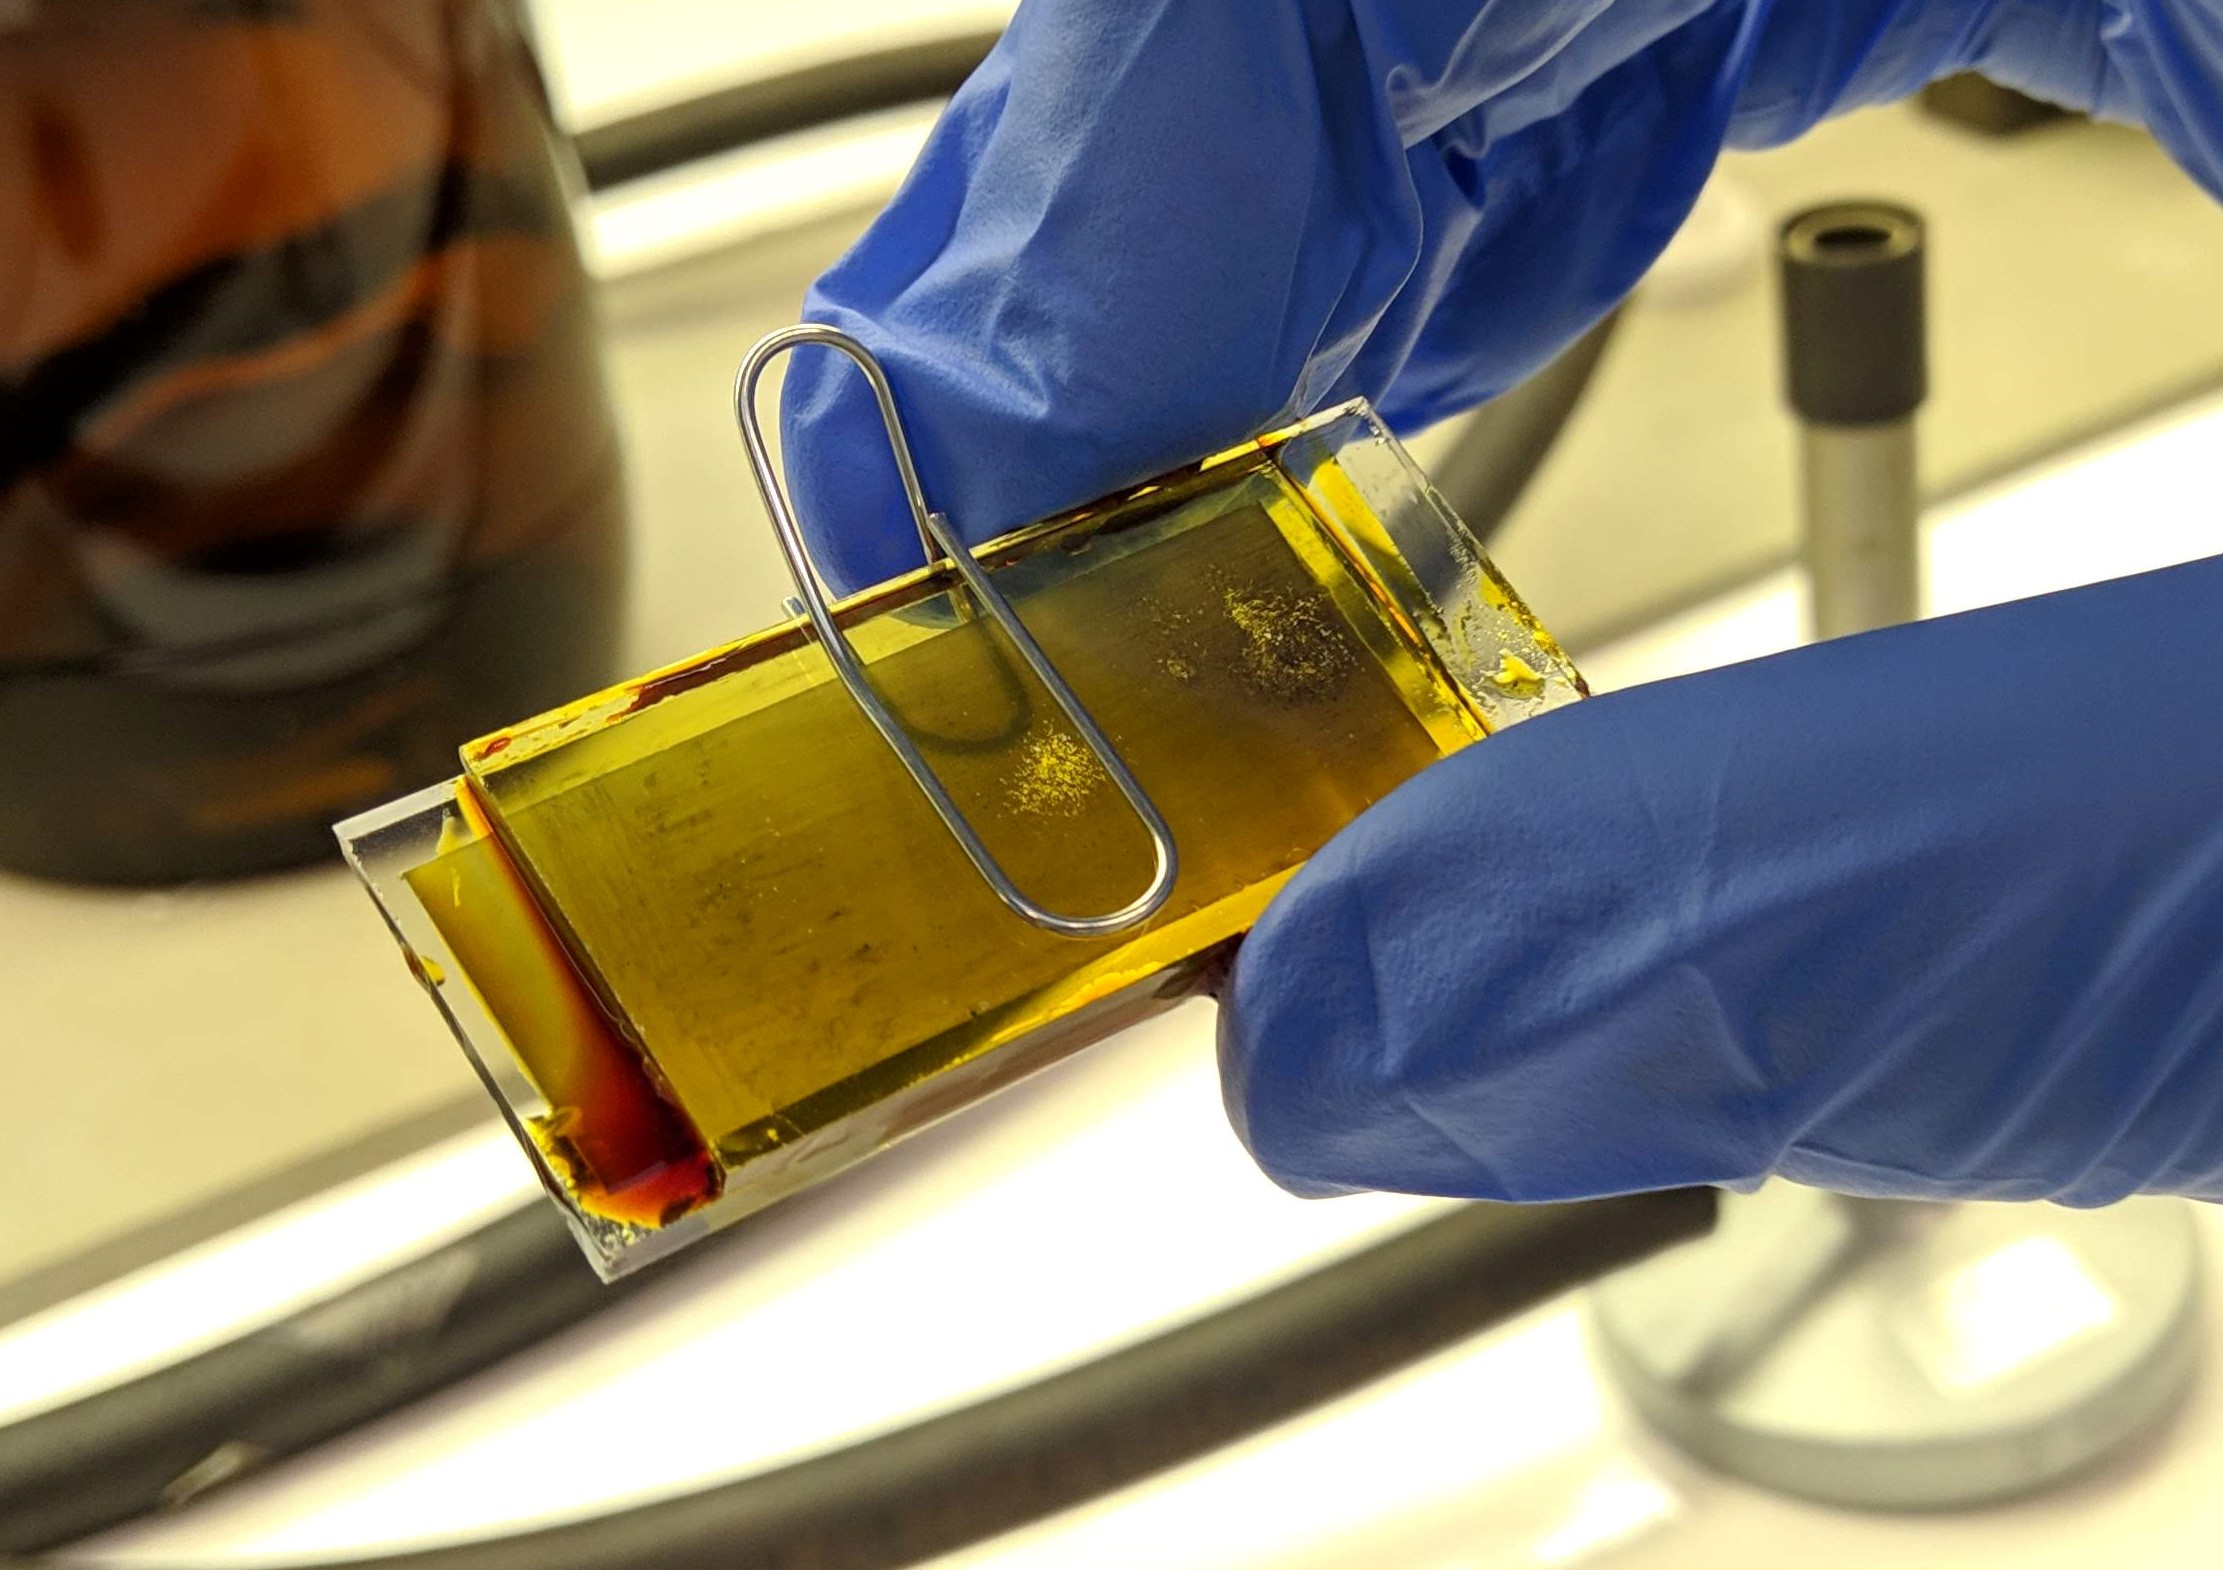
\includegraphics[width=0.35\textwidth]{10ElectroliteAndClamped.jpg}
\caption{The final result for the Hibiscus dye solar cell.}
\label{fig:resultsolarcell} %use label to refer to it in later text
\end{figure}

\subsubsection{Testing the cells}
First, the solar cell was connected to the measuring equipment (multimeter) to make sure there was no short circuit. The solar cell was tested in two conditions: with and without external light. For the measurement without light, the surrounding light was blocked with hands. The measurement with light was done with an external light source directly above the solar cell. Before starting IV measurement, the anode (positive electrode) was connected to the red cable (+), the cathode (negative electrode) was connected with the black cable (-) and calibration is also necessary. A voltage ranging from -2V to 2V over the solar cell was applied. The current from multimeter was noted down and this data was put in the LabView program. After the measurement was done the data was saved for further calculations.

\section{Results}
In this section, the assembly process is discussed. The IV measurements are calculated and compared to another groups' measurements. We took the group that also used beetroot to compare our results because it is the same dye. Polyfit was used in Excel to return the coefficients for a polynomial of degree 6 that is the best fit for the gathered data for our calculations. Take note that a polynomial fit introduces a small error for values. For each dye the Zero Current, Short Current and Power are calculated.\\

\subsection{Cell Assembly}
As seen in figure \ref{fig:resultteabeet} there are some imperfections in the resulting solar cells. The black tea dye left some tiny black tea leaf particles attached to the TiO$_2$ paste which could influence the efficiency. The bottom picture shows that a whole area of TiO$_2$ paste was flushed away during the rinsing process, reducing efficiency.
For the Hibiscus solar cell, an open-circuit voltage ($V_{OC}$) of 0.427V was measured, the beetroot had a $V_{OC}$ of 0.285V and the black tea had a $V_{OC}$ of 0.320V.\\

\begin{figure}[H]
\centering
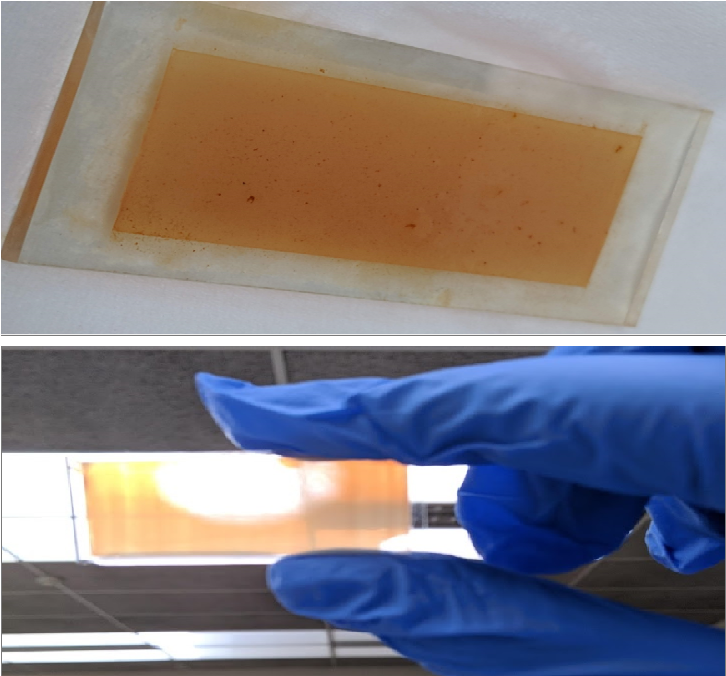
\includegraphics[width=0.35\textwidth]{combined.png}
\caption{Imperfections of the solar cells}
\label{fig:resultteabeet} %use label to refer to it in later text
\end{figure}
\subsection{Calculations}

\subsubsection{Equations}
The equation for power is \begin{equation} \label{eq:power} P = UI \end{equation}
Equations for our data:
The equation for beetroot with a $R^2$ of 0.0995 with no light is: 
\begin{equation} \label{eq:redbeetnolighteq} 
\begin{aligned}
f_{NLB}(x) = -0.0551x^6 - 0.072x^5 + 0.3559x^4 + 0.7374x^3 +\\ 0.2129x^2 -0.1846x - 0.0419
\end{aligned}
\end{equation}

\noindent The equation for beetroot with a $R^2$ of 0.0993 with light is: 
\begin{equation} \label{eq:redbeetlighteq}
\begin{aligned}
f_{LB}(x) = -0.0419x^6 - 0.083x^5 + 0.2468x^4 + 0.7848x^3 +\\ 0.5164x^2 - 0.0428x - 0.1076
\end{aligned}
\end{equation}

\noindent The equation for black tea with a $R^2$ of 0.09988 with no light is: 
\begin{equation} \label{eq:blackteanolighteq} 
\begin{aligned}
f_{NLBT}(x) = -0,0248x^6 - 0,0472x^5 + 0,2539x^4 + \\0,6834x^3 + 0,3401x^2 - 0,1366x - 0,0589
\end{aligned}
\end{equation}

\noindent The equation for black tea with a  $R^2$ of 0.09987 with light is: 
\begin{equation} \label{eq:blacktealighteq} 
\begin{aligned}
f_{LBT}(x) = -0,0429x^6 - 0,0721x^5 + 0,2769x^4 + \\0,6217x^3 + 0,1821x^2 - 0,1242x - 0,0239
\end{aligned}
\end{equation}

\noindent Equations for other student data:

\noindent The equation for other groups' beetroot with a $R^2$ of 0.09989 with no light is: 
\begin{equation} \label{eq:otherredbeetlighteq} 
\begin{aligned}
f_{ONLB}(x) = -0,0461x^6 - 0,0676x^5 + 0,3087x^4 +\\ 0,6825x^3 + 0,2151x^2 - 0,1781x - 0,0467
\end{aligned}
\end{equation}

\noindent The equation for other groups' beetroot with a $R^2$ of 0.09987 with light is: 
\begin{equation} \label{eq:otherredbeetlighteq} 
\begin{aligned}
f_{OLB}(x) = -0,005x^6 - 0,0587x^5 - 0,0039x^4 +\\ 0,5028x^3 + 0,6885x^2 + 0,1667x - 0,1332
\end{aligned}
\end{equation}


\subsubsection{Zero Current}
Zero current is the value where the graph intersects with the y-axis $(x = 0)$.
Given equations \ref{eq:redbeetnolighteq}, \ref{eq:redbeetlighteq}, \ref{eq:blackteanolighteq} and \ref{eq:blacktealighteq} filling in $(x = 0)$ gives:
\begin{itemize}
 \item$f_{NLB}(0)$ : -0.0419 mA
 \item$f_{LB}(0)$ : -0.1076 mA
 \item$f_{NLBT}(0)$: -0,0589 mA
 \item$f_{LBT}(0)$: -0,0239 mA
 \item$f_{ONLB}(0)$: -0,0467 mA
 \item$f_{OLB}(0)$: -0,1332 mA
\end{itemize}
\subsubsection{Short Current}
Short current is the value where the graph intersects with the x-axis $(y = 0)$ where $x \in [-2, 2]$ (see section Testing the cells).
Given equations \ref{eq:redbeetnolighteq}, \ref{eq:redbeetlighteq}, \ref{eq:blackteanolighteq} and \ref{eq:blacktealighteq} filling in $(y = 0)$ gives:
\begin{itemize}
 \item$(f_{NLB}(x) = 0, x)$ : 0.04532 mA
 \item$(f_{LB}(x) = 0, x)$ : 0.382537 mA
 \item$(f_{NLBT}(x) = 0, x)$: 0.00 mA
 \item$(f_{LBT}(x) = 0, x)$: 0.3959 mA
 \item$(f_{ONLB}(x) = 0, x)$: 0.01 mA
 \item$(f_{OLB}(x) = 0, x)$: 0.3108 mA
\end{itemize}

\subsubsection{Max Power}
The maximum power can be found by calculating the maximal surface below the curve. This point $P$ can be found by finding the maximum value for $x_1$ * $y_1$. This gives an equation $f_{max}$ = $x_1 * f(x_1)$. Using equation $(\frac{d}{dx} f_{max} = 0 , x)$ gives a value for P where the area is maximal (taking the second derivative $\frac{d^2}{dx^2}$ gives a minimal because of the negative y).\\This gives a value for voltage (V) and current (mA) representing each value for the surface as seen in fig \ref{fig:powercalc}.
\begin{figure}[H]
\centering
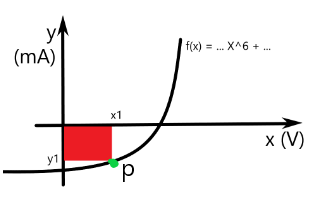
\includegraphics[width=0.45\textwidth]{powercalc2.png}
\caption{Calculating the maximal power.}
\label{fig:powercalc} %use label to refer to it in later text
\end{figure}
Using previously explained reasoning we get the point x for maximal power for each solar cell (with and without light) as follows:\\
solve($(\frac{d}{dx}(x*f_{cell}(x) = 0,x)$)$|0<x<2$
\begin{itemize}
 \item$f_{NLB}(x)$ : x = 0.30248
 \item$(f_{LB}(x)$ : x = 0.23340
 \item$(f_{NLBT}(x))$: x = 0.26813
 \item$(f_{LBT}(x)$: x = 0.26334
 \item$(f_{ONLB}(x)$: x = 0.310978
 \item$(f_{OLB}(x))$: x = 0.175693
\end{itemize}
Applying these values to equation \ref{eq:power} using previously found point x.
\begin{itemize}
 \item$P_{NLB} = 0.30V * 0.30* 10^{-3} A$ = 90 $\mu W$
 \item$P_{LB} = 0.23V * 0.23* 10^{-3} A$ = 52.9 $\mu W$
 \item$P_{NLBT} = 0.27V * 0.27* 10^{-3} A$ = 72.9 $\mu W$
 \item$P_{LBT} = 0.26V * 0.26* 10^{-3} A$ = 67.6 $\mu W$
 \item$P_{ONLB} = 0.31V * 0.31* 10^{-3} A$ = 96.1 $\mu W$
 \item$P_{OLB} = 0.175V * 0.175* 10^{-3} A$ = 30.6 $\mu W$ 
\end{itemize}

 
\begin{figure}[H]
\centering
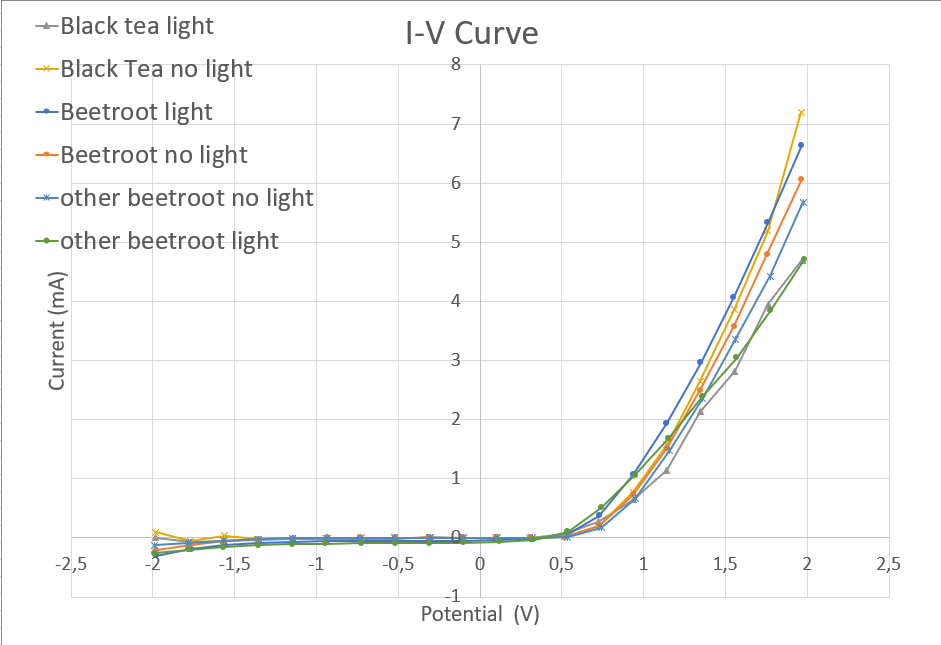
\includegraphics[width=0.45\textwidth]{IVCURVE.png}
\caption{Results for the IV measurements for our beetroot, black tea and another groups' beetroot.}
\label{fig:redbeetcurve} %use label to refer to it in later text.
\end{figure}

\subsection{Discussion}

It came to our attention that both the beetroot in this experiment and the beetroot of our fellow students have about the same power output when there is no light (90 $\mu W$, 96.1  $\mu W$) but varies when there is light. Further, some results with the light on have lower power output than their non-light variant. This may be because of the inaccuracy of the measurement setup or the polyfit approximation error. Also, it is noticeable that the output power is very minimal (near zero). This could be because of bad quality dye, fabrication errors or bad glass conductivity.\\

When comparing the efficiencies from the research, it was mentioned that beetroot had an efficiency of 1.30 \% and black tea had an efficiency of 0.20 \%. One would expect that the maximal power would be linear with the efficiency thus beetroot having a significantly bigger maximal power. However,  a maximal power for beetroot (with light) of 52.9 $\mu W$ and for black tea 67.6 $\mu W$ was measured, contradicting this statement. A reason for this could be because when the beetroot TiO$_2$ paste cell was taken out of the petri dish, a large blank area was noticed (see figure \ref{fig:resultteabeet}). This affects the area of paste, reducing efficiency.\\

When measuring the initial range was set from -1V to 2V. However, this gave no result when running the measurement LabView program. The range had to be adjusted to -2V to 2V in order to get data. A reason for this could be the bad conductivity of the glass plate.

\section{Conclusion}
Making TiO$_2$ dye-sensitized solar cells can be done easily with a natural dye which can be found in a kitchen. The process is, however, a delicate process where the smallest error can influence the efficiency a lot (one of the cells had a blank spot due to rinsing).\\
The dyes were chosen with their according efficiency regarding the found literature. However, our results did not represent those of the literature study. The reasons could be faulty equipment, a bad glass plate or a bad dye.\\
The calculations were done by polyfitting the data into 6th order functions. This also introduces an error which could influence the made calculations. However, during the calculations we calculated another groups' maximal power as well, using the same dye (beetroot) and concluded an almost linear trend.


\begin{thebibliography}{00}

\bibitem{monomulti} T. Schoder, 'Monocrystalline Cells vs. Polycrystalline Cells: What's the Difference?', civicsolar, 2018. [Online]. Available: \url{https://www.civicsolar.com/article/monocrystalline-cells-vs-polycrystalline-cells-whats-difference} [Accessed: 03- Nov- 2019]

\bibitem{redturnipeff} O. Adedokun, K. Titilope, A. O. Awodugba ``Review on Natural Dye-Sensitized Solar Cells (DSSCs)'' INTERNATIONAL JOURNAL of ENGINEERING TECHNOLOGIES, Oluwaseun Adedokun et al., Vol.2, No.2, 2016

\bibitem{redbeeteff} S. Sathyajothi, R. Jayavel,A. Clara Dhanemozhi ``Fabrication of Natural Dye Sensitized Solar Cell (Dssc) based on TiO2 Using Henna And Beetroot Dye Extracts'' 5th International Conference of Materials Processing and Characterization (ICMPC 2016)

\bibitem{betalinpicture} Raja Ramamoorthy, Natarajan Radha, Govindaraj Maheswari, Sambandam Anandan, Subbaiah Manoharan, Rayar Victor Williams ``Betalain and anthocyanin dye-sensitized solar cells'' J Appl Electrochem
DOI 10.1007/s10800-016-0974-9

\bibitem{blacktea} N. T. R. N. Kumara, M. R. Rahimi Kooh, A. Lim,
M. I. Petra, N. Y. Voo, C. M. Lim, and P. Ekanayake ``DFT/TDDFT and Experimental Studies of Natural Pigments Extracted from Black Tea Waste for DSSC Application'' Hindawi Publishing Corporation
International Journal of Photoenergy, Volume 2013, Article ID 109843, 8 pages


\bibitem{15naturaldyes} M. Abdel-latif, M. Abruiriban, N. Al-Dahoudi ''Dye-Sensitized Solar Cells Using Fifteen Natural Dyes as Sensitizers of Nanocrystalline TiO2'' [Online]. Available: \url{https://www.researchgate.net/publication/282239122_Dye-Sensitized_Solar_Cells_Using_Fifteen_Natural_Dyes_as_Sensitizers_of_Nanocrystalline_TiO2} [Accessed: 13- Nov- 2019]

\end{thebibliography}
\end{document}